%---------------------------------------------------------------
\chapter{Experiments}
%---------------------------------------------------------------
\label{ch:experiments}

\section{Data}
\subsection{ReKIS}

\textit{Regionales Klimainformationssystem Sachsen, Sachsen-Anhalt, Thüringen} -- ReKIS -- is a regional climate information system operating in Central Germany. 
We will use its product \textit{KlimRefDS\_v3.1\_1961-2023}, which monitors several climate variables from 1961 to 2023.
This dataset will be used for training purposes in LR and HR pairs, where the LR images will be resampled from this HR dataset.

\begin{figure}[htbp]
    \centering
    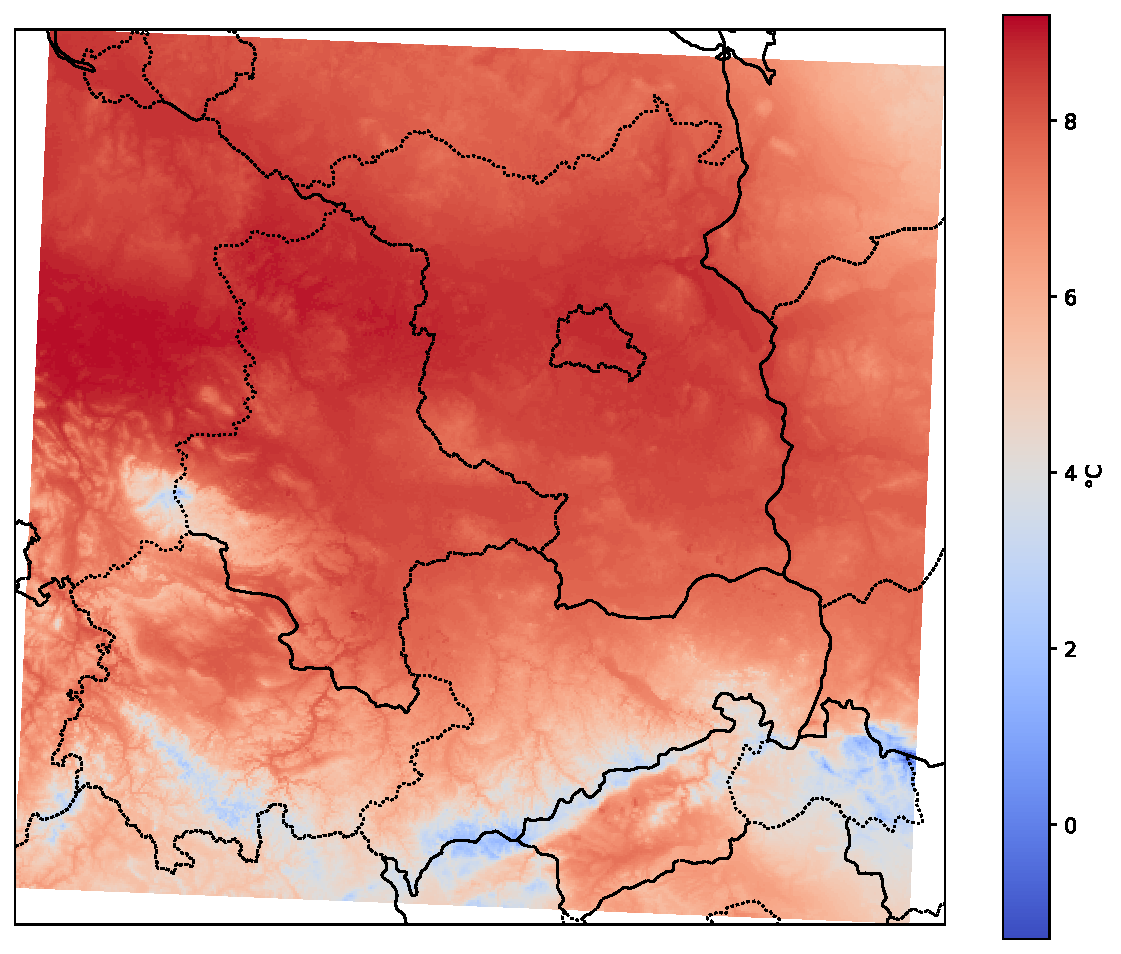
\includegraphics[width=0.7\linewidth]{images/rekis.pdf}
    \caption[ReKIS example]{ReKIS example. The mean temperature on 2000-02-01 is shown.}
    \label{fig:rekis_2000_02_01}
\end{figure}

\begin{description}
    \item[Region.] The studied region is Central Germany, mainly the area of the constituent states of Saxony, Saxony-Anhalt, and Thuringia. 
    This region does not form a square on the map; therefore, data from other neighboring German constituent states, Poland, and Czechia were included. 
    \item[Variables.] The data collected consist of multiple climate variables, which are listed in Table~\ref{tab:ReKISdata}.
    These variables are present in daily, monthly, and annual means.
    In this work, we will focus on daily mean temperature.
    \item[Grid.] Data were obtained from observational meteorological stations.
    From these stations, ReKIS produced grids for each variable using interpolation, in the form displayed in Figure~\ref{fig:rekis_2000_02_01}.
\end{description}

{
\shorthandoff{-}
\begin{table}[htbp]
    \centering
    \begin{tabular}{|l|c|l|}
        \hline
        \textbf{Variable name}              & \textbf{Unit} & \textbf{Note} \\ 
        \hline
        Vapor pressure                     & $\text{hPa}$ & Daily mean \\ 
        \hline
        Saturation vapor pressure          & $\text{hPa}$ & Daily mean \\ 
        \hline
        \multirow{2}{*}{Potential evaporation}              & $\text{mm} \cdot \text{day}^{-1}$ & Daily sum \\ 
        \cline{2-3}
        & $\text{W} \cdot \text{m}^{-2}$ & Daily mean \\         
        \hline
        Mean wind speed                    & $\text{m} \cdot \text{s}^{-1}$ & Daily mean \\ 
        \hline
        Maximum wind speed                 & $\text{m} \cdot \text{s}^{-1}$ & Daily maximum \\ 
        \hline
        \multirow{2}{*}{Grass reference evapotranspiration} & $\text{mm} \cdot \text{day}^{-1}$ & Daily sum \\ 
        \cline{2-3}
        & $\text{W} \cdot \text{m}^{-2}$ & Daily mean \\ 
        \hline
        Relative humidity                  & $\text{\%}$ & Daily mean \\ 
        \hline
        \multirow{2}{*}{Global solar radiation} & $\text{J} \cdot \text{cm}^{-2}$ & Daily sum \\ 
        \cline{2-3}
        & $\text{W} \cdot \text{m}^{-2}$ & Daily mean \\ 
        \hline
        Corrected precipitation            & $\text{mm} \cdot \text{day}^{-1}$ & Daily sum \\ 
        \hline
        Uncorrected precipitation          & $\text{mm} \cdot \text{day}^{-1}$ & Daily sum \\ 
        \hline
        Mean temperature                   & $^\circ\text{C}$ & Daily mean \\ 
        \hline
        Minimum temperature                & $^\circ\text{C}$ & Daily minimum \\ 
        \hline
        Maximum temperature                & $^\circ\text{C}$ & Daily maximum \\ 
        \hline
    \end{tabular}
    \caption[ReKIS climate variables]{ReKIS climate variables.}
    \label{tab:ReKISdata}
\end{table}
}

The area covered by ReKIS is predominantly flat in its northern and central parts, while its southern section is characterized by mountainous terrain.
The high elevation also influences the mean temperature, which is visible both in the one day mean Figure~\ref{fig:rekis_2000_02_01} and in Figure~\ref{fig:rekis_mean}, which depicts the mean temperature from 1961 to 1992.
It is clear that the HR structures and distinct boundaries, particularly the warm temperature corridors in mountainous areas, are also retained in the mean temperature field.
These are characteristics that cannot be completely captured in LR images, and the models will need to handle them accordingly.

\begin{figure}[htbp]
    \centering
    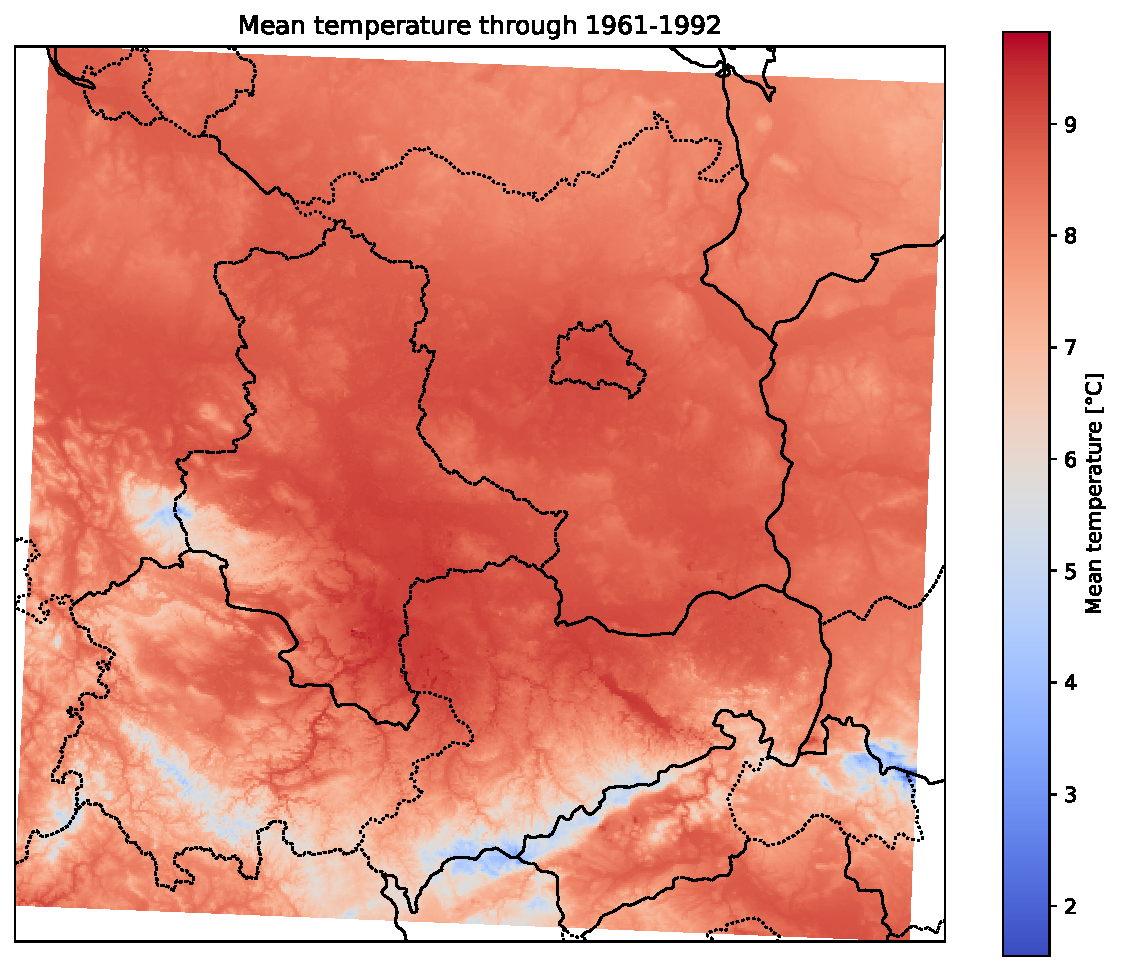
\includegraphics[width=0.7\linewidth]{images/rekis_mean.pdf}
    \caption[ReKIS mean temperature through 1961--1992]{ReKIS mean temperature through 1961--1992.}
    \label{fig:rekis_mean}
\end{figure}

\subsection{EURO-CORDEX}

The European Coordinated Downscaling Experiment -- EURO-CORDEX -- as its name suggests, is an ensemble of regional climate downscaling experiments~\cite{Jacob2014}.
One of them is REMO2015, an experiment where the regional climate model REMO was run on the boundary conditions of the global climate model ERA-Interim reanalysis.
We will use this experiment, more specifically its evaluation version (where the model was run on past conditions), with a resolution of $0.11^\circ$ (12.5 km) from the years 1979 to 2012.
This experiment covers the whole of Europe and provides several climate variables; however, we will use only daily mean temperature.
For the sake of simplicity, we will refer to this dataset as the EURO-CORDEX dataset in this work, even though it is only a small fraction of the EURO-CORDEX example and even from the REMO2015 experiment.
An example is shown in Figure~\ref{fig:cordex}.

\begin{figure}
    \centering
    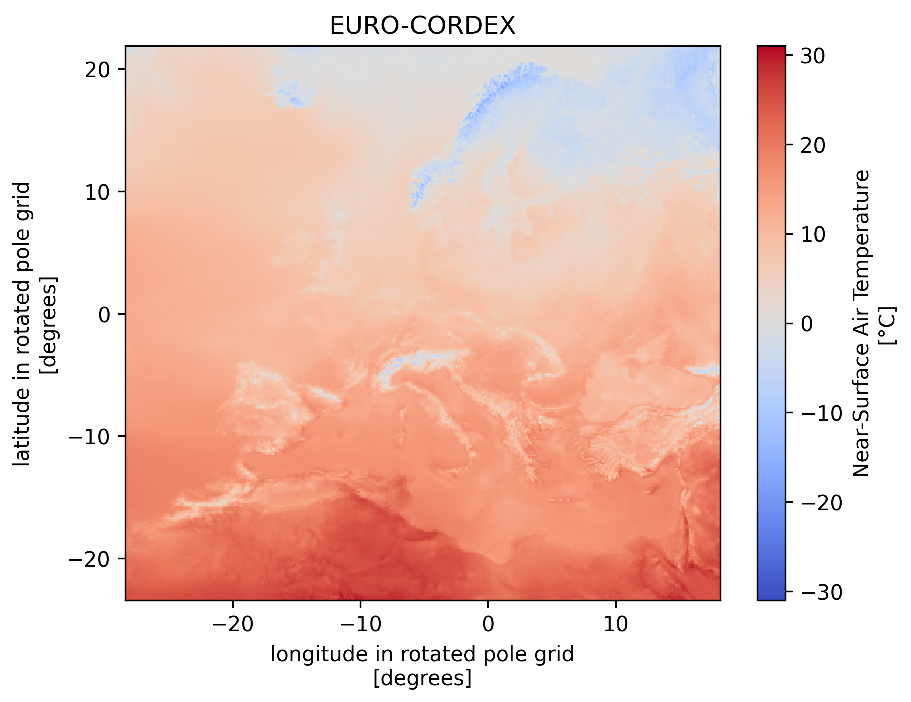
\includegraphics[width=0.8\linewidth]{images/cordex.pdf}
    \caption[EURO-CORDEX example]{EURO-CORDEX example. The mean temperature on 2000-02-01 is shown.}
    \label{fig:cordex}
\end{figure}

\subsection{Workflow}

Our primary goal is to downscale the climate projections (EURO-CORDEX).
However, those do not have a HR version.
Therefore, we incorporate the observational gridded dataset (ReKIS), where the HR data are available.
Then we produce LR images from them using a resampling method and train the model on these observational LR and HR pairs.
We also evaluate the models on the observational data and choose the best one, which will be applied to LR projections, yielding the final HR predictions.
This process is visualized in Figure~\ref{fig:workflow}.

\begin{figure}
    \centering
    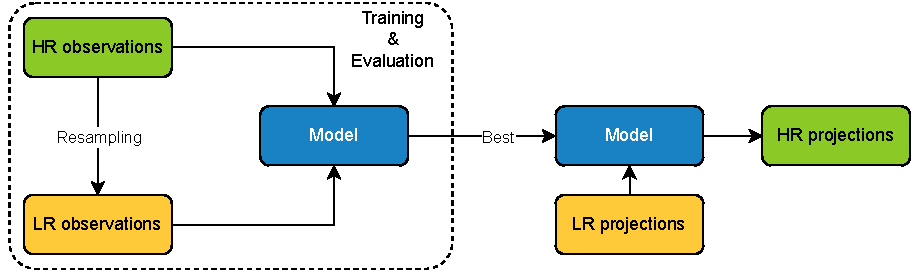
\includegraphics[width=\linewidth]{images/workflow.pdf}
    \caption[Workflow]{Workflow. Initially the model is trained on the observations, which are available in HR version, and can be resampled to LR version. We evaluate and choose the best model on the observations. Then we apply the best model to LR predictions. The LR data are highlighted in yellow, the HR in green and the models in blue.}
    \label{fig:workflow}
\end{figure}

\subsection{Data preprocessing}

For the work with geospatial data, we used the rioxarray package.
ReKIS and the EURO-CORDEX data have different coordinate reference systems (CRS).
ReKIS uses the 3-degree Gauss-Kruger zone 4, whereas EURO-CORDEX uses the World Geodetic System 1984.
We will reproject the EURO-CORDEX data to match ReKIS's CRS.

The grid from ReKIS was cropped to $400 \times 400$ HR images.
These images are then downsampled to a lower resolution to generate the LR images, which are divided into three groups by year: a training set (1961--1992), a validation set (1993--2002), and a test set (2003--2012).
The division by years is to simulate the predictions of the model on unseen data, which can have a different distribution than the observed ones.
We restrict ourselves to ReKIS data up to 2012, even though data are available through 2023, because we also need to retain unseen data within the EURO-CORDEX dataset.


\section{Resampling method}
\label{s:resampling_method_exp}

Before any training can take place, it is necessary to have LR and HR pairs prepared.
The HR parts are from ReKIS, and the LR parts need to be obtained by resampling the HR images.
However, there are more methods for such transformation -- nearest, bilinear, cubic, cubic spline, Lanczos, and average resampling.
The differences are visible in the example of the mean temperature on 2000-02-01 in Figure~\ref{fig:resampling}.
The smoothest LR image appears to be the one generated by cubic spline, whereas the one with the highest changes between its neighbors is generated by the nearest resampling.
The concept of dilated derivative consistency applies exclusively to resampling methods that can be expressed as a convolution with a fixed kernel; among the methods mentioned, only average resampling fulfills this requirement.
Košťál et al.~\cite{Kostal2025} applied cubic spline, whereas Harder et al.~\cite{Harder2023} referred to average resampling as the ``standard methodology in climate downscaling studies''.
The upcoming Sections (\ref{ss:performance_resampling} and \ref{ss:violation_resampling}) will examine which is the most advantageous for our specific use case.

\begin{figure}[htbp]
    \centering
    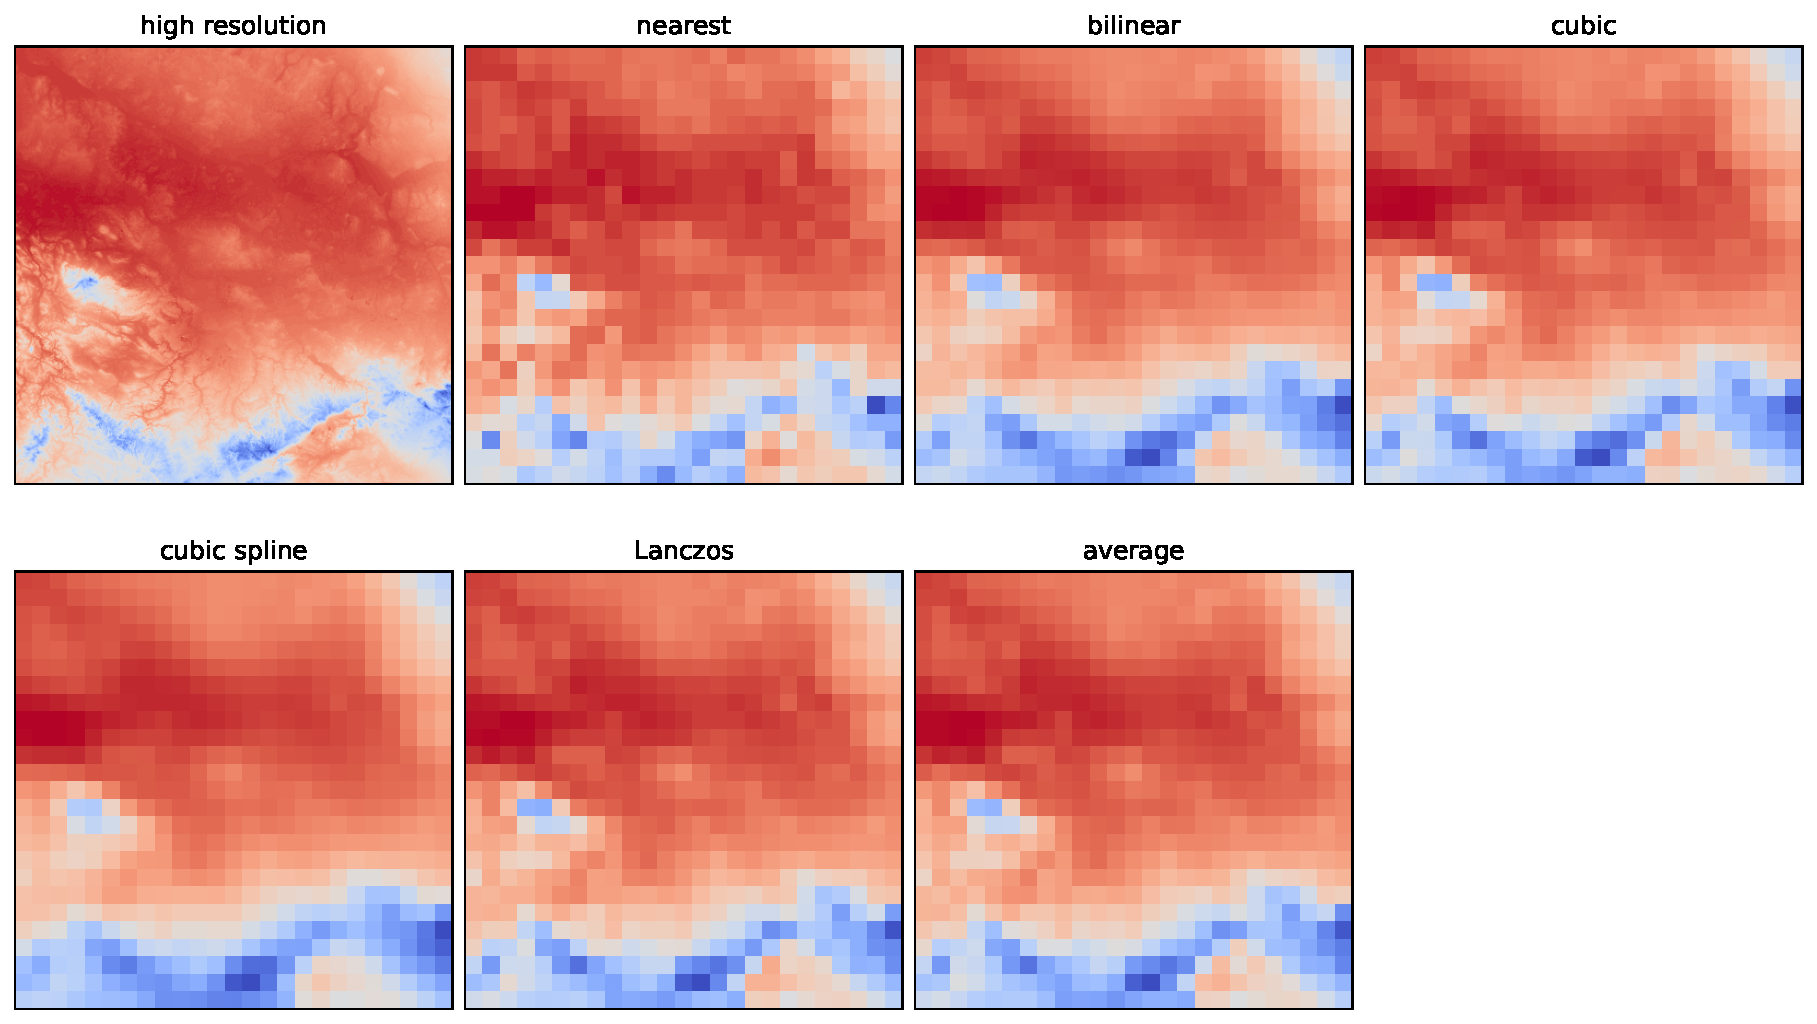
\includegraphics[width=\linewidth]{images/resampling.pdf}
    \caption[Resampling methods]{Resampling methods. The original HR image is shown on the left top of the figure, then six examples of resampling -- nearest, bilinear, cubic, cubic spline, Lanczos, and average -- have been applied on it. The results of resampling the HR image with scale factor of 16 are shown. The HR image from ReKIS shows mean temperature on 2000-02-01.}
    \label{fig:resampling}
\end{figure}

\subsection{Model performance orientated choice of resampling method}
\label{ss:performance_resampling}

One approach to decide which resampling method will be used is to measure the model performance on both resampling methods.
For better comparison, we include more scale factors and an unconstrained model, a soft-constrained model, and a hard-constrained model.
For the model, we choose EDSR with 128 residual blocks and 64 features, exactly as in the best model by Košťál et al.~\cite{Kostal2025}.
As representatives of both soft and hard constraints, we use the conservation law, since it is the only constraint in this work that can be implemented both ways. 
Therefore, the focus will be on the implementation, not on the appropriateness of the physical principle.
As the conservation soft constraint version, we choose squared, and the $\alpha$ parameter equal to $10^{-4}$, both the same as Harder et al.~\cite{Harder2023}.
Hard constraining is implemented as an additive constraint layer because it performs the best among the three possibilities (Section~\ref{s:hard_constraint_exp}). 
We include both cubic spline and average pooling, used by Košťál et al.~\cite{Kostal2025} and Harder et al.~\cite{Harder2023}.

All the results are shown in Figure~\ref{fig:scale_factor_model_type}.
Much new information can be observed there.
First, when using hard constraints with the cubic spline, the performance was significantly worse than both the average resampling scenario and the other types of constraints applied in the cubic spline setting.
This can be caused by the fact that the hard constraining layer is enforcing a relation -- conserving the mean through downscaling -- that is not present even between LR and target HR images, as will be shown in Section~\ref{ss:violation_resampling}.
Next, the hard constraint using the average resampling method was applied across all scale factors within the best configurations, also shown in Table~\ref{tab:best_for_scale_factor}. 
Moreover, the final configuration demonstrated a stabilizing effect on model performance as the scale factor increased, whereas the other configurations exhibited greater volatility.
Starting from a scale factor of 40, the model’s RMSE values began to rise sharply.
Yet, even at this scale, the input LR image is only $10 \times 10$, while the model generates SR images of size $400 \times 400$.
In other words, the model must infer $1600$ SR pixels from a single LR pixel, which is understandably challenging and contributes to the increased error produced by the model.

\begin{figure}[htbp]
    \centering
    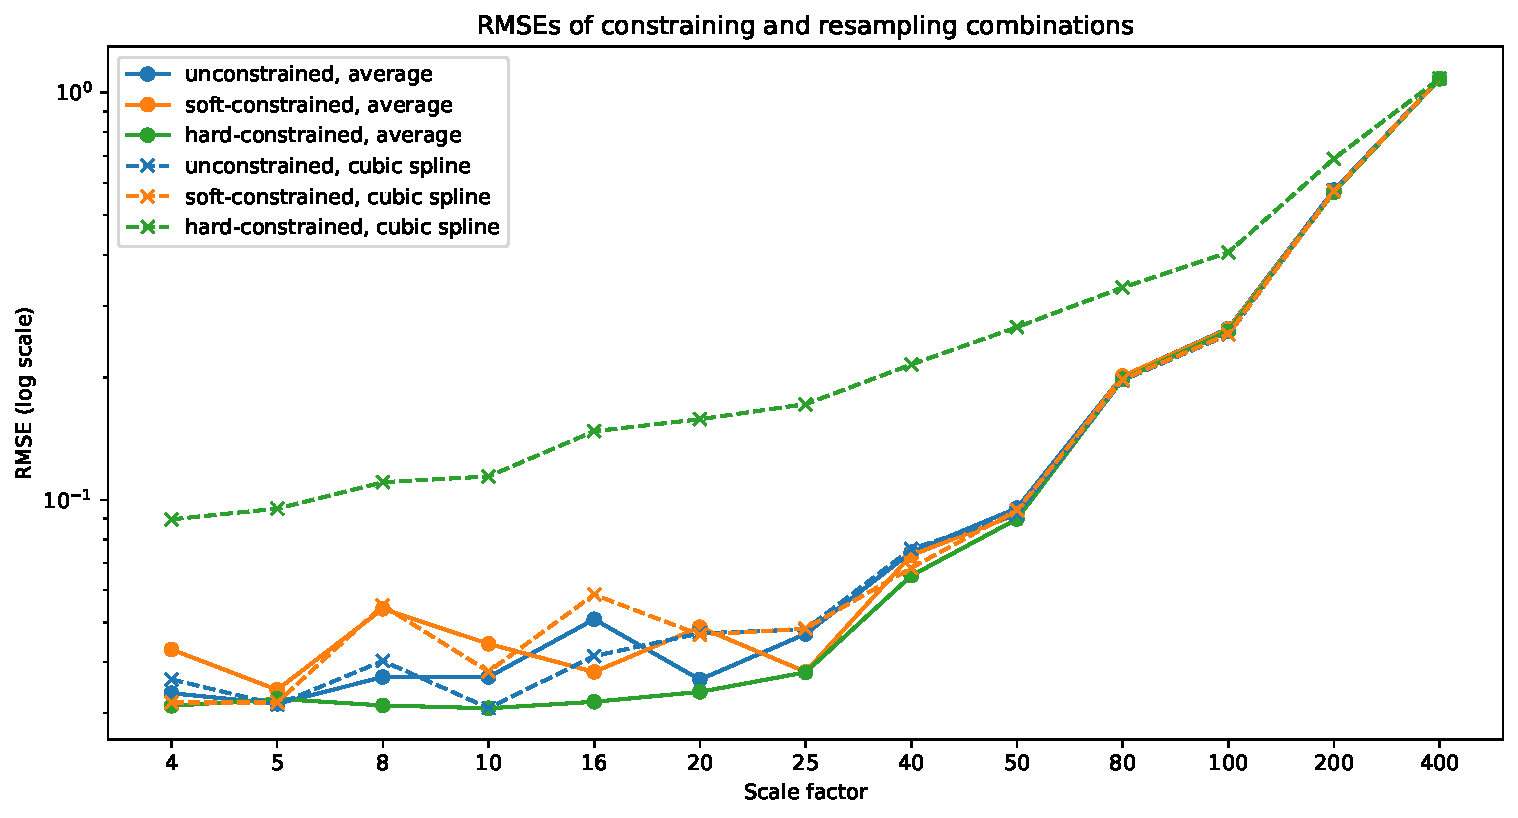
\includegraphics[width=\linewidth]{images/resampling_plot.pdf}
    \caption[Scale factor and model types performances]{Scale factor and model types performances.}
    \label{fig:scale_factor_model_type}
\end{figure}

\begin{table}[htbp]
    \centering
    \begin{tabular}{|c|l|c|c|}
        \hline
         \textbf{scale factor} &  \textbf{RMSE} & \textbf{resampling method} & \textbf{constraining} \\
         \hline \hline
         $4\times$ & 0.0312 & average & hard \\ \hline 
         $5\times$ & 0.03142 & cubic spline & unconstrained \\ \hline 
         $8\times$ & 0.03128 & average & hard \\ \hline 
         $10\times$ & 0.03078 & average & hard \\ \hline 
         $16\times$ & 0.03193 & average & hard \\ \hline 
         $20\times$ & 0.03377 & average & hard \\ \hline 
         $25\times$ & 0.03772 & average & hard \\ \hline 
         $40\times$ & 0.06515 & average & hard \\ \hline 
         $50\times$ & 0.08976 & average & hard \\ \hline 
         $80\times$ & 0.19673 & cubic spline & unconstrained \\ \hline 
         $100\times$ & 0.25454 & cubic spline & unconstrained \\ \hline 
         $200\times$ & 0.57030 & average & hard \\ \hline 
         $400\times$ & 1.08279 & average & hard \\ \hline 
    \end{tabular}
    \caption[Best models for each scale factor]{Best model type and resampling method pairs are shown for each scale factor.}
    \label{tab:best_for_scale_factor}
\end{table}

Focusing on the improvement of the constrained models with respect to the unconstrained one, it is evident that using average resampling, the majority of runs yielded better results when the hard constraint was present (Figure~\ref{fig:res_rel_avg}).
Exactly the opposite can be observed in the cubic spline case, where the hard constrained models have shown worse performance than the unconstrained versions (Figure~\ref{fig:res_rel_cs}).
In both settings, soft constraining shows balancing ratios on the edge of improvement.
The most significant improvement was achieved for the hard constrained model with average resampling downscaling with a scale factor of 16.

\begin{figure}[htbp]
    \centering
    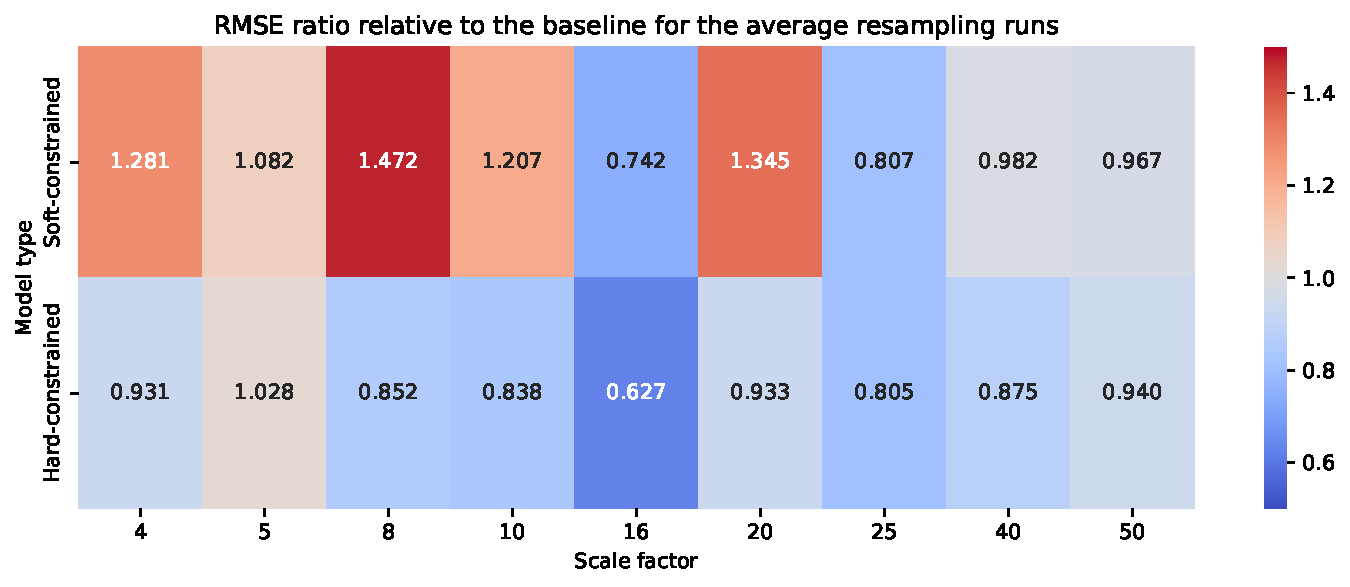
\includegraphics[width=0.75\linewidth]{images/resampling_rel_avg_9.pdf}
    \caption[Relative model improvement across scale factors in the average resampling setting]{Relative model improvement across scale factors in the average resampling setting.}
    \label{fig:res_rel_avg}
\end{figure}

\begin{figure}[htbp]
    \centering
    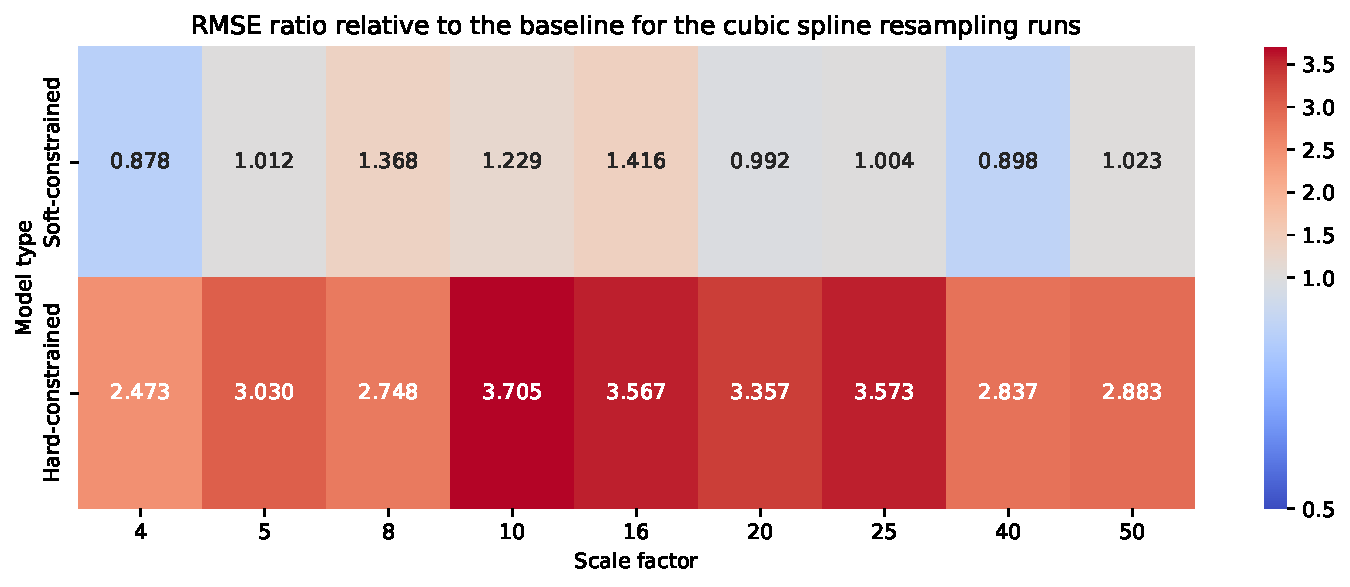
\includegraphics[width=0.75\linewidth]{images/resampling_rel_cs_9.pdf}
    \caption[Relative model improvement across scale factors in the cubic spline resampling setting]{Relative model improvement across scale factors in the cubic spline resampling setting. Note that the color palette is non-linear; it has been adjusted so that the blue values indicate improvement relative to the corresponding baseline model.}
    \label{fig:res_rel_cs}
\end{figure}

\subsection{Target violation orientated choice of resampling method}
\label{ss:violation_resampling}

The fundamental property of a constraint should be that the violation is equal to zero for LR and HR pairs.
That is the best a hypothetical model could achieve when trained under a particular constraint. 
Therefore, we will calculate the mean violation for each constraint on the train ReKIS dataset.
The results are visible in Table~\ref{tab:resampling_soft_exp}.
It is clearly visible that average pooling dominates other methods and confirms the role of ``standard methodology''~\cite{Harder2023}.
In the remainder of this work, average pooling will be implicitly adopted as the resampling method, as it achieved the best performance in both experiments.

\begin{landscape}
{
\shorthandoff{-}
\begin{table}[htbp]
    \centering
    \begin{tabular}{|l|c|l|l|l|l|l|l|}
        \hline
        \textbf{Constraint name} & \textbf{Version} & \textbf{nearest} & \textbf{bilinear} & \textbf{cubic} & \textbf{cubic spline} & \textbf{Lanczos} & \textbf{average} \\ 
        \hline
        \hline
        \multirow{2}{*}{Conservation law} & absolute & 0.13428 & 0.03583 & 0.0225 & 0.07657 & 0.03859 & \textbf{0.00001} \\ 
        \cline{2-8}
        & squared & 0.05433 & 0.00387 & 0.00137 & 0.01738 & 0.00402 & \textbf{0} \\
        \hline
        \multirow{2}{*}{Simple derivative} & absolute & 0.38241 & 0.1024 & 0.0609 & 0.2038 & 0.10007 & \textbf{0} \\ 
        \cline{2-8}
        & squared & 0.21994 & 0.01661 & 0.00563 & 0.06648 & 0.01475 & \textbf{0}  \\       
        \hline
        \multirow{2}{*}{Sobel gradient magnitude} & absolute & 0.48015 & 0.14631 & 0.08667 & 0.35088 & 0.17259 & \textbf{0} \\ 
        \cline{2-8}
        & squared & 0.63199 & 0.06462 & 0.01989 & 0.37543 & 0.08638 & \textbf{0}  \\       
        \hline
        \multirow{2}{*}{Continuity} & absolute & 0.16535 & 0.06096 & 0.00156 & 0.12777 & 0.0341 & \textbf{0} \\ 
        \cline{2-8}
        & squared & 0.3045 & 0.09947 & 0.00484 & 0.19380 & 0.06993 & \textbf{0} \\         
        \hline
        \multirow{2}{*}{G-Loss} & absolute & 0.19072 & 0.0511 & 0.03032 & 0.10464 & 0.05038 & \textbf{0} \\ 
        \cline{2-8}
        & squared & 0.10876 & 0.00825 & 0.00273 & 0.03446 & 0.00735 & \textbf{0} \\        
        \hline
        \multirow{2}{*}{Simple gradient direction} & absolute & 0.07963 & 0.00476 & 0.00285 & 0.01708 & 0.00636 & \textbf{0} \\ 
        \cline{2-8}
        & squared & 0.04772 & 0.00058 & 0.00015 & 0.00471 & 0.00062 & \textbf{0} \\        
        \hline
        \multirow{2}{*}{Sobel gradient direction} & absolute & 0.09696 & 0.00477 & 0.00222 & 0.02248 & 0.00683 & \textbf{0} \\ 
        \cline{2-8}
        & squared & 0.09551 & 0.00037 & 0.00008 & 0.00646 & 0.00068 & \textbf{0} \\        
        \hline
    \end{tabular}
    \caption[Resampling and soft constraints]{Resampling and soft constraints. For each constraint type, six resampling methods are evaluated by measuring the violation between the HR image and the resampled LR image. The best result for each soft constraint is shown in \textbf{bold}. From these experiments, average pooling clearly emerges as the most effective resampling technique among those tested.
    Note that this outcome is expected: when average resampling is used, derivative consistency holds (Section~\ref{ss:dilated_sr_derivative}), leading to identical derivatives. 
    As a result, the constraints cannot penalize any difference between them.
    The values were rounded to 5 decimal places.
    }
    \label{tab:resampling_soft_exp}
\end{table}
}
\end{landscape}

\section{Hard constraint type}
\label{s:hard_constraint_exp}

As shown in Equations~\eqref{e:hard_constraint_layers}, there are three types of hard constraint layers: additive, multiplicative, and soft-max layer.
We will conduct an experiment to determine which one will be used further on.

The results in Table~\ref{tab:hard_constraint_implementation} indicate that the multiplicative method performs significantly worse than the other two approaches. 
Moreover, the soft-max variant still exhibits an RMSE that is more than twice as large as that of the additive layer.
We consider this to be a huge difference, and in this work, we will always use the additive implementation.

\begin{table}[htbp]
    \centering
    \begin{tabular}{|l|l|l|}
        \hline
         \textbf{Type} & \textbf{MAE} & \textbf{RMSE} \\
         \hline \hline
         additive & \textbf{0.02603} & \textbf{0.0315} \\
         \hline
         multiplicative & 0.14764 & 0.25448 \\
        \hline
        soft-max & 0.03481 & 0.07369 \\
        \hline
    \end{tabular}
    \caption[Hard constraint layer implementation experiment]{Hard constraint layer implementation experiment.}
    \label{tab:hard_constraint_implementation}
\end{table}

Both the multiplicative and soft-max constraint layers encounter difficulties when the mean temperature is near 0$^\circ$C because of the division involved (Equations~\eqref{e:hard_constraint_layers}).
In addition, the soft-max layer preserves the sign of the LR pixel across all of its corresponding downscaled pixels.
Yet, 0$^\circ$C does not have a special thermodynamic significance like 0K, so preserving the sign in this way is not particularly beneficial.

\section{Soft constraint type}
\label{s:constraints_exp}

Initially, we analyze how each soft constraint affects the models' performance.
We follow Košťál et al.~\cite{Kostal2025} and, as the model type, we choose EDSR with 64 channels and 128 residual blocks.
We use the constraint loss ratio $\alpha = 10^{-4}$, the same as the best value used by Harder et al.~\cite{Harder2023}.
In each experiment, we choose a constraint and a type of penalty, and train the model above with this configuration. 
The scale factor applied in this experiment is the one for which the constraining yielded the greatest improvement (Section~\ref{ss:performance_resampling}) -- namely, $16\times$.

The results are shown in Table~\ref{tab:soft_constraints_exp}.
The best constraint was the one penalizing the difference in the derivatives calculated by the simple kernels.
The second best was the modified G-Loss constraint.
There is no consistent dominance of any version of the interested constraints.
All the runs have produced reasonable results.

{
\shorthandoff{-}
\begin{table}[htbp]
    \centering
    \begin{tabular}{|l|c|l|l|}
        \hline
        \textbf{Constraint name} & \textbf{Version} & \textbf{MAE} & \textbf{RMSE} \\ 
        \hline
        \hline
        \multirow{2}{*}{Conservation law} & absolute & 0.03776 & 0.05392 \\ 
        \cline{2-4}
        & squared & 0.0278 & 0.0378 \\         
        \hline
        \multirow{2}{*}{Simple derivative} & absolute & \textbf{0.02709} & \textbf{0.0358} \\ 
        \cline{2-4}
        & squared & 0.04662 & 0.06364 \\         
        \hline
        \multirow{2}{*}{Sobel gradient magnitude} & absolute & 0.0304 & 0.0432 \\ 
        \cline{2-4}
        & squared & 0.04159 & 0.0594 \\         
        \hline
        \multirow{2}{*}{Continuity} & absolute & 0.03032 & 0.04301 \\ 
        \cline{2-4}
        & squared & 0.04211 & 0.0583 \\         
        \hline
        \multirow{2}{*}{G-Loss} & absolute & \textit{0.02762} & \textit{0.03750} \\ 
        \cline{2-4}
        & squared & 0.03812 & 0.05429 \\         
        \hline
        \multirow{2}{*}{Simple gradient direction} & absolute & 0.0452 & 0.06299 \\ 
        \cline{2-4}
        & squared & 0.03959 & 0.05652 \\         
        \hline
        \multirow{2}{*}{Sobel gradient direction} & absolute & 0.05167 & 0.07144 \\ 
        \cline{2-4}
        & squared & 0.03071 & 0.04287 \\         
        \hline
    \end{tabular}
    \caption[Constraint types experiment]{Constraint types experiment. Best result is highlighted in \textbf{bold}, the second best in \textit{italics}.}
    \label{tab:soft_constraints_exp}
\end{table}
}

\section{Soft constraint alpha value}
\label{s:soft_constraints_alpha_exp}

We conduct a simple search for the optimal $\alpha$ for the best constraint type from Section~\ref{s:constraints_exp} -- the absolute version of the simple derivative constraint.
The $\alpha$ value, as described in Equation~\eqref{e:soft_constraint}, determines the relative influence of the constraint with respect to the pixel-wise loss.

Results are shown in Table~\ref{tab:alpha_exp}.
It is evident that placing excessive emphasis on minimizing the constraint violation (high $\alpha$) over pixel-wise loss is not improving the model's performance.
The best alpha value was $10^{-4}$, the same as in Harder et al.~\cite{Harder2023}; however, this is a different constraint with possibly a different range.
Moreover, it is clearly demonstrated that including a certain amount of physical information, with the weight $\alpha$ in the range of $10^{-5}$ to $10^{-2}$, has a beneficial impact compared to a model that relies only on a pixel-wise loss function ($\alpha = 0$).

\begin{table}[htbp]
    \centering
    \begin{tabular}{|l|l|l|}
        \hline
         $\mathbf{\alpha}$ & \textbf{MAE} & \textbf{RMSE} \\
         \hline
         \hline
         1 & 2.91212 & 4.2134 \\
         \hline
         0.99999 & 2.82308 & 4.08568 \\
         \hline
         0.9999 & 0.33783 & 0.65158 \\
         \hline
         0.999 & 0.18782 & 0.31223 \\
         \hline
         0.99 & 0.16098 & 0.27225 \\
         \hline
         0.9 & 0.03794 & 0.05481 \\
         \hline
         0.5 & 0.0291 & 0.04008 \\
         \hline
         0.1 & 0.03978 & 0.05556 \\
         \hline
         0.01 & 0.05832 & 0.08171 \\
         \hline
         0.001 & \textit{0.0281} & \textit{0.03862} \\
         \hline
         0.0001 & \textbf{0.02709} & \textbf{0.0358} \\
         \hline
         0.00001 & 0.02975 & 0.04134 \\
         \hline
         0 & 0.03569 & 0.05092 \\
         \hline
    \end{tabular}
    \caption[Soft constraining alpha experiments]{Soft constraining alpha experiments. Best results are highlighted in \textbf{bold}, the second best in \textit{italics}.}
    \label{tab:alpha_exp}
\end{table}

\section{Model size}
\label{s:models_size_exp}

We study how the model size -- the number of the model's trainable parameters -- affects its performance.
The question of size arises from the usage of the smaller SRCNN in Harder et al.~\cite{Harder2023} compared to the larger EDSR in Košťál et al.~\cite{Kostal2025}.
We inspect EDSR model types with $r \in\{ 1, 2, 4, 8, 16, 32, 64, 128 \}$ residual blocks and $f \in\{ 1, 2, 4, 8, 16, 32, 64, 128 \}$ features -- channels used in residual blocks -- for unconstrained, soft conservation constraint, and hard conservation constraint.
The conservation constraint is chosen because it is the only one in this work that has both soft and hard constraint implementations, allowing us to compare the two approaches.
All the models will perform downscaling with a scale factor of 16.

The EDSR model size is dependent on the previously stated number of residual blocks $r$ and the number of channels $f$ used in those.
First, in a convolutional layer with a kernel size of $k \times k$ and $c_{in}$ input channels, $c_{in}$ different kernels are used for the convolution with the $c_{in}$ input channels, after that an element-wise sum is calculated and a bias is added, producing one of $c_{out}$ output channels.
This corresponds to the overall number of parameters being:
\begin{equation}
    p_\text{CL} = \left(k^2 \cdot c_{in} + 1\right) \cdot c_{out}.
\end{equation}
Throughout all the EDSR convolutional layers, only a kernel size of $3 \times 3$ is used.
The head of the EDSR model consists of a single convolutional layer, the task of which is to produce $f$ channels from the single input channel. 
Thus, the number of parameters in the head is equal to:
\begin{equation}
    p_\text{head} = \left(3^2 \cdot 1 + 1\right) \cdot f = 10f.
\end{equation}
In the body, firstly $r$ residual blocks are present, each with two convolutional layers with $f$ input and $f$ output channels.
After them an additional convolutional layer is used with the same configuration.
The number of learnable parameters in the body is:
\begin{equation}
    p_\text{body} = \left(3^2 \cdot f + 1\right) \cdot f \cdot (2r + 1) = 18f^2r + 9f^2 + 2fr + f.
\end{equation}
In the tail, the upsampling takes place.
For each prime factor $p_i$ of scale factor $s$ a convolutional layer with $f$ input channels and $f\cdot p_i^2$ output channels is employed, followed by a pixel shuffle layer, which does not have any learnable parameters and only reshapes its input to have $f$ channels again.
After the upsampler, the last convolution takes place, where the $f$ channels are converted into single one.
Using the scale factor equal to $16 = 2^4$, the number of learnable parameters in the tail is:
\begin{equation}
    p_\text{tail} = \left(3^2 \cdot f + 1\right) \cdot f \cdot 2^2 \cdot 4 + \left( 3^2 \cdot f + 1 \right) \cdot 1 = 144f^2 + 25f + 1
\end{equation}
Making in total:
\begin{equation}
    \begin{aligned}
        p_\text{EDSR} &= p_\text{head} + p_\text{body} + p_\text{tail} \\
        &= 10f + 18f^2r + 9f^2 + 2fr + f + 144f^2 + 25f + 1 \\
        &= 18f^2r + 153f^2 + 2fr + 36f + 1
    \end{aligned}
    \label{e:edsr_size}
\end{equation}
learnable parameters.
From this point, it is obvious that the size will grow faster with respect to the number of features than to the number of residual blocks.
Using the Equation~\eqref{e:edsr_size} we calculated the sizes of each model configuration used in this experiment (Table~\ref{tab:sizes}).
The wide range from hundreds to 40 million learnable parameters will be enough to observe how the model size influences the performances of the unconstrained, soft-constrained, and hard-constrained models.

{
\shorthandoff{-}
\begin{table}[htbp]
    \centering
    \begin{tabular}{|cc|c|c|c|c|c|c|c|c|}
        \hline
         & & \multicolumn{8}{c|}{residual blocks} \\
         & & 1 & 2 & 4 & 8 & 16 & 32 & 64 & 128 \\
         \hline
         \multirow{8}{*}{\rotatebox[origin=c]{90}{features}} 
         & 1 & 210 & 230 & 270 & 350 & 510 & 830 & 1.5K & 2.8K \\
         \cline{2-10}
         
          & 2 & 761 & 837 & 989 & 1.3K & 1.9K & 3.1K & 5.5K & 10K \\
         \cline{2-10}
          & 4 & 2.9K & 3.2K & 3.8K & 5K & 7.3K & 12K & 22K & 40K \\
         \cline{2-10}
          & 8 & 11K & 12K & 15K & 19K & 29K & 47K & 85K & 160K \\
         \cline{2-10}
          & 16 & 44K & 49K & 58K & 77K & 114K & 188K & 337K & 634K \\
         \cline{2-10}
          & 32 & 176K & 195K & 232K & 306K & 454K & 750K & 1.3M & 2.5M \\
         \cline{2-10}
          & 64 & 703K & 777K & 924K & 1.2M & 1.8M & 3M & 5.4M & 10M \\
         \cline{2-10}
          & 128 & 2.8M & 3.1M & 3.7M & 4.9M & 7.2M & 12M & 21M & 40M \\
         \hline
    \end{tabular}
    \caption[Number of parameters in EDSR models]{Number of parameters in EDSR models.}
    \label{tab:sizes}
\end{table}
}

The results of this experiment are shown in Figure~\ref{fig:sizes}.
Across all three model types, larger model sizes were associated with lower RMSE values.
Similar to increasing the scale factor in the average resampling scenario in Figure~\ref{fig:scale_factor_model_type}, the hard-constrained model's performance appears to be more balanced than the noisier results of the unconstrained and soft-constrained models. 
In the experiments, the RMSE spans a fairly broad range, from $0.032$ to $0.307$, which aligns with a wide range of model sizes employed.

\begin{landscape}
    \begin{figure}
    \centering
    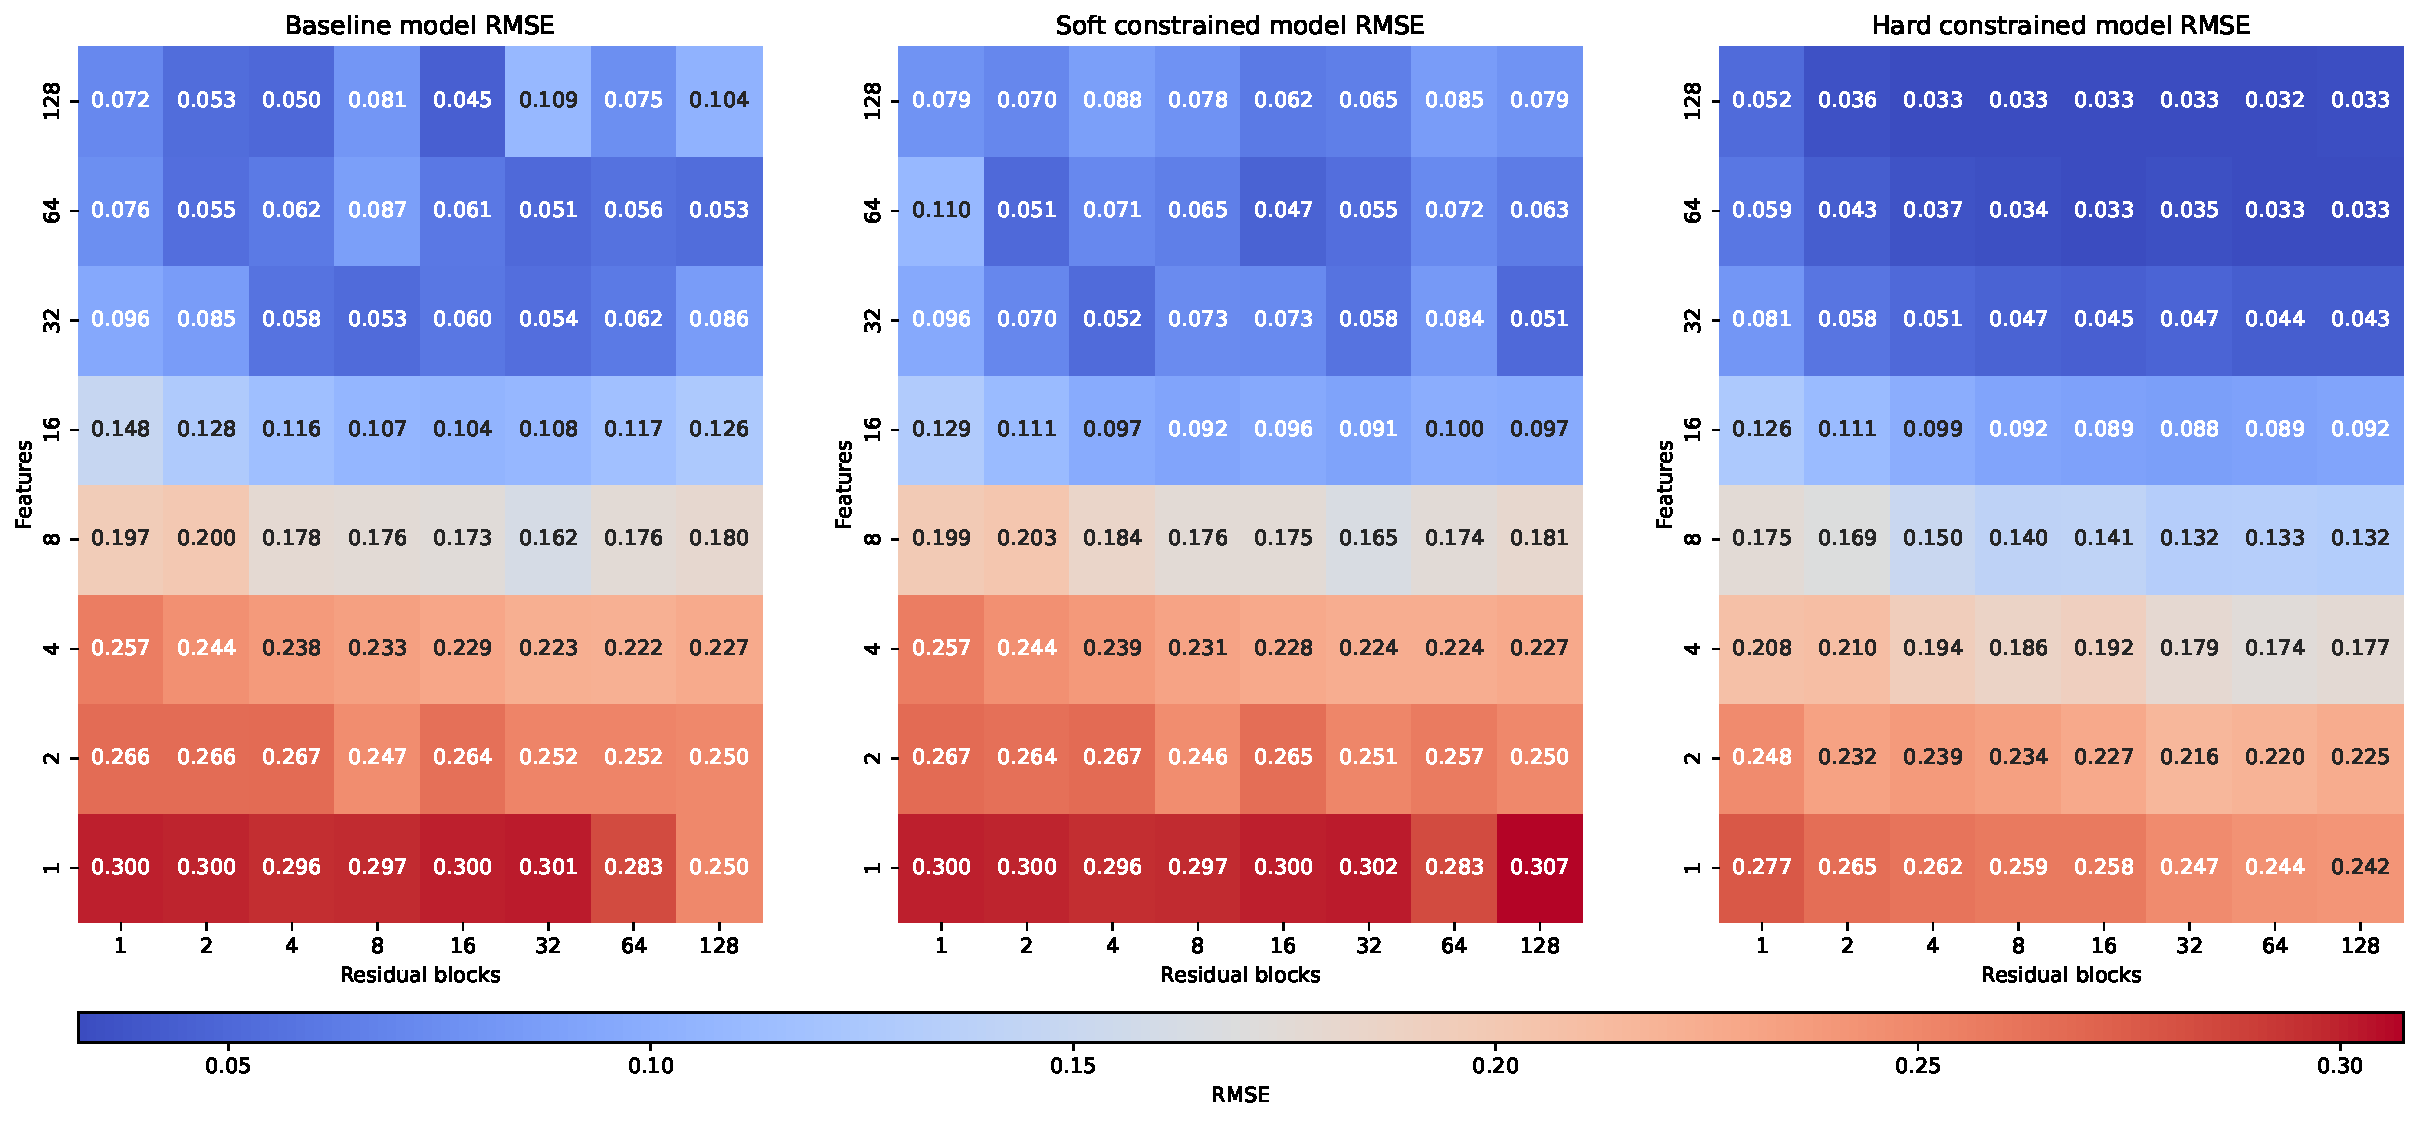
\includegraphics[width=\linewidth]{images/sizes.pdf}
    \caption[Model size experiment]{Model size experiment result. From left to right the RMSEs achieved by unconstrained, soft-constrained and hard-constrained models.}
    \label{fig:sizes}
\end{figure}
\end{landscape}

The absolute differences between the RMSEs of unconstrained models and both soft and hard constrained models are shown in Figure~\ref{fig:sizes_abs_diff}.
For the soft constraint scenario, in the smaller model sizes, the results are comparable to the unconstrained models, except for one case that appears to be random noise.
For the configuration with 16 features, the soft-constrained models consistently yield better performance for every tested number of residual blocks.
Beginning with 32 features and above, the results fluctuate between improvement and deterioration. 
This behavior can be explained by the large pixel-wise error for the small model sizes, forcing the model to focus on that part of the loss function, leading to the same results as the unconstrained models.
For the 16 features, the pixel-wise error drops, and the ratio between it and the constraint violation appears to be ideal.
When the number of features reaches 32 or more, the results for both the unconstrained and soft-constrained models become turbulent. 
This may be due to the low pixel-wise loss, suggesting that the model is overfitted.
On the other hand, the hard constraint scenario shows RMSE improvement across all the model sizes.

\begin{figure}[h]
    \centering
    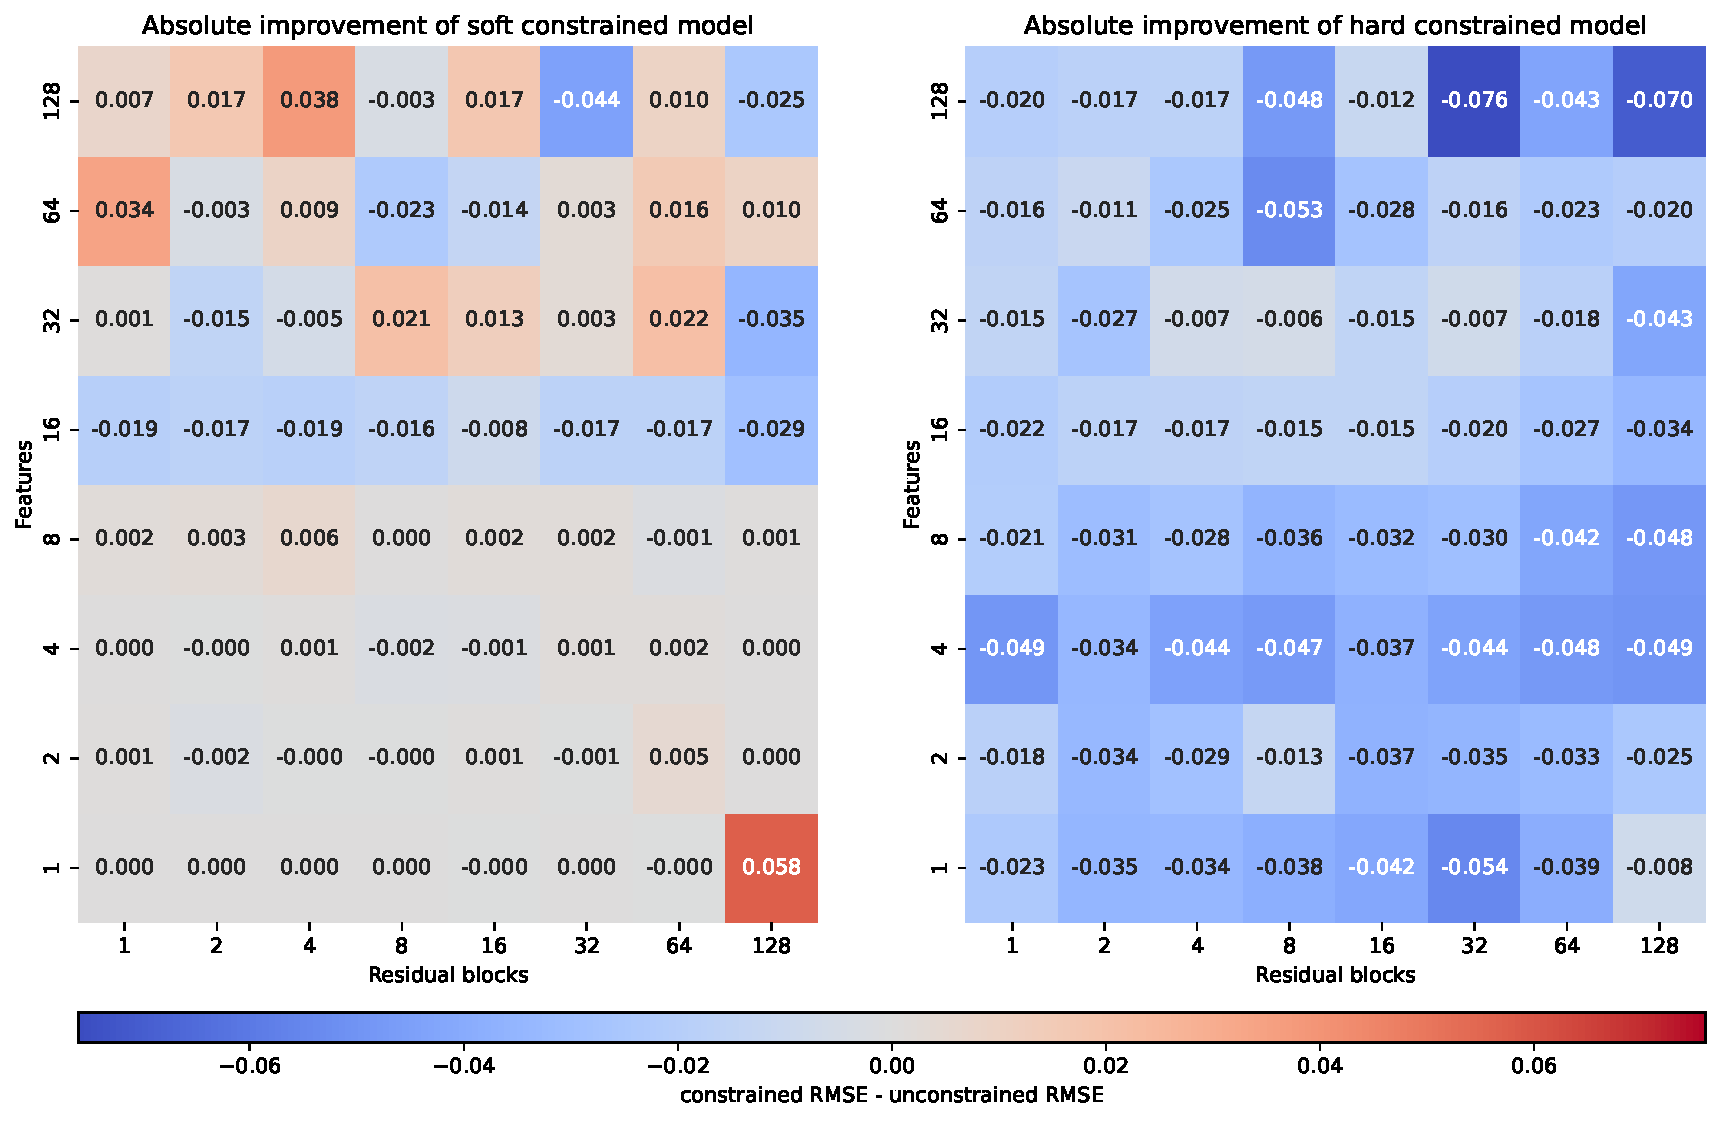
\includegraphics[width=\linewidth]{images/sizes_abs_diff.pdf}
    \caption[Model size experiment -- absolute improvement]{Model size experiment -- absolute improvement. The differences between RMSEs of unconstrained model and soft-constrained (left), resp. hard-constrained (right) models of the same size are shown. When the model's performance improved by incorporating a constraint the value is negative and is displayed in blue, otherwise in red.}
    \label{fig:sizes_abs_diff}
\end{figure}

When focusing on relative improvements (Figure~\ref{fig:sizes_rel_diff}) of the soft and hard constrained models in comparison with their unconstrained counterparts, the conclusions from the previous paragraph remain valid.
Moreover, together with the smoothing effect of the hard constraints shown in Figure~\ref{fig:sizes} and the observation that the relative improvement grows with model size, we conclude that the hard constraint layer contributes to generalization.

\begin{figure}[h]
    \centering
    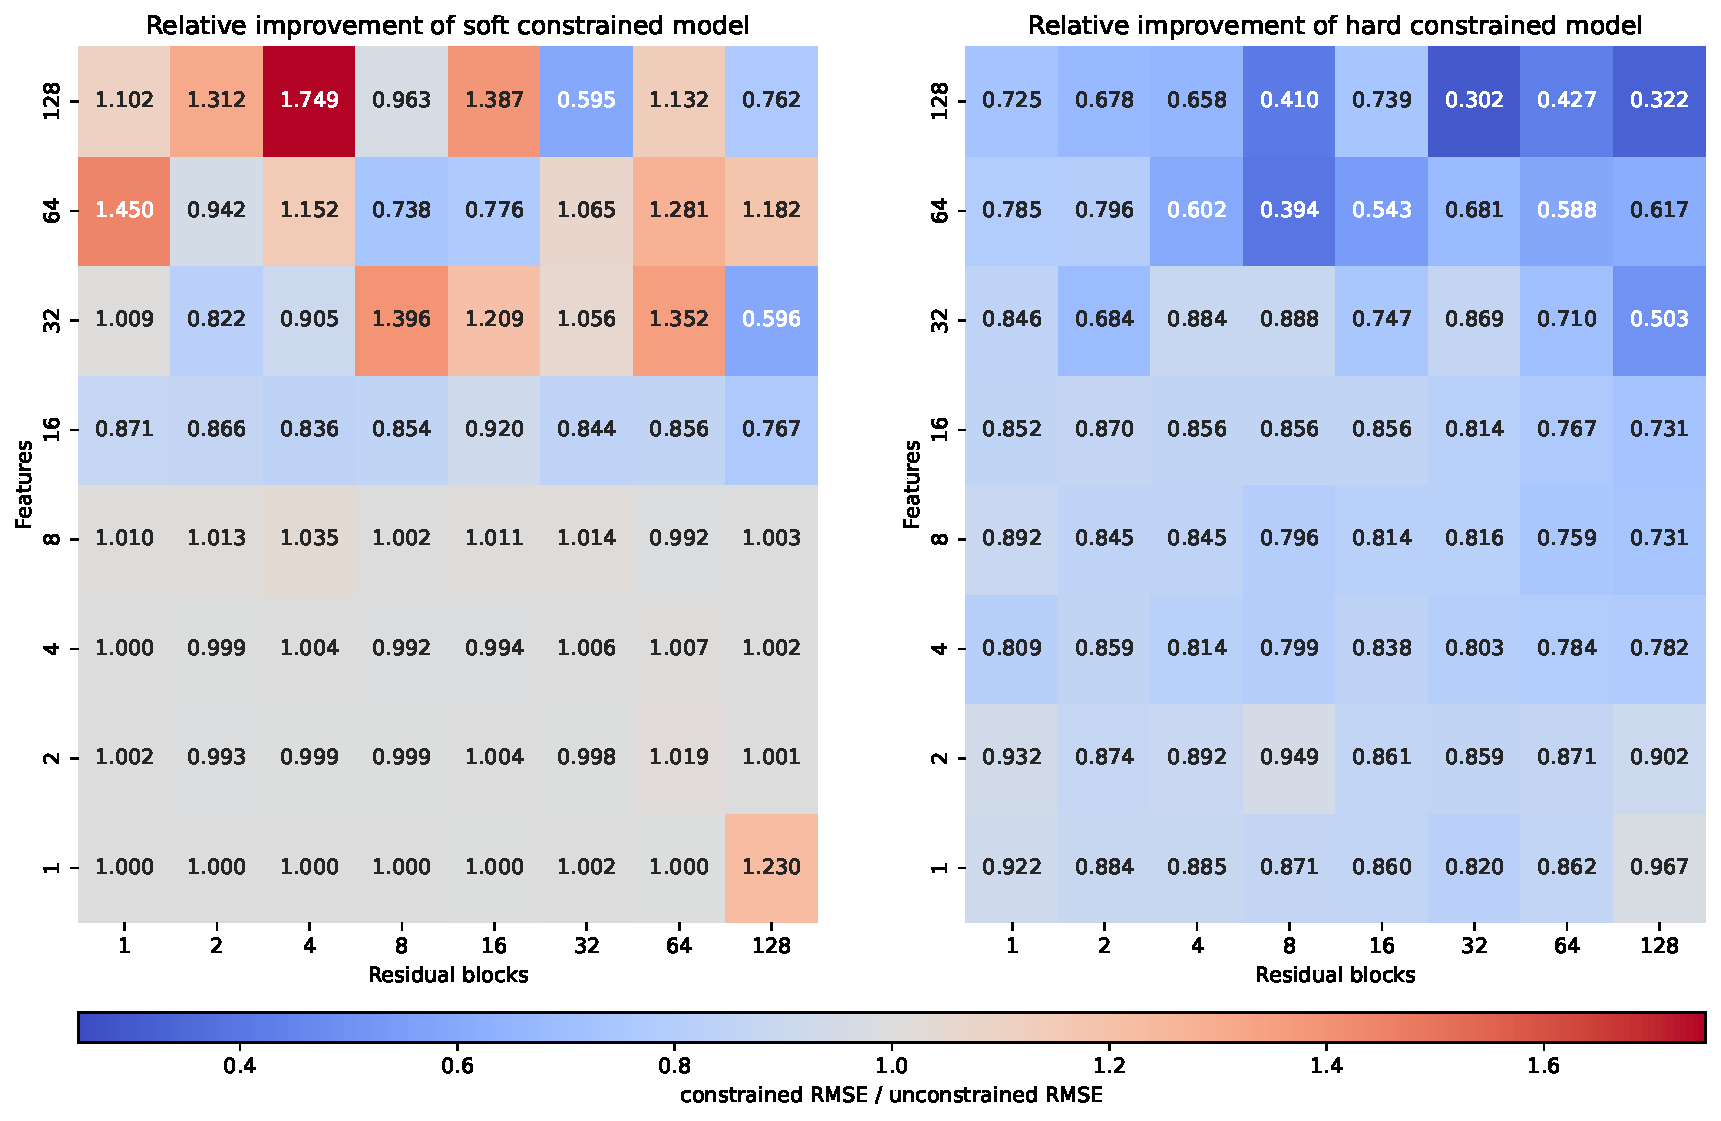
\includegraphics[width=\linewidth]{images/sizes_rel_diff.pdf}
    \caption[Model size experiment -- relative improvement]{Model size experiment -- relative improvement. The ratios between RMSEs of unconstrained model and soft-constrained (left), resp. hard-constrained (right) models of the same size are shown. When the model's performance improved by incorporating a constraint the value is less than one and is displayed in blue, otherwise in red.}
    \label{fig:sizes_rel_diff}
\end{figure}

The lowest RMSE obtained (0.03223) was achieved by the hard-constrained model using 64 residual blocks and 128 features. 
The best performance of the unconstrained model (0.04456) was slightly better than that of the soft-constrained model (0.04702).
That leads us to the conclusion that the hard-constraining layer reduced the pixel-wise error of the unconstrained model by almost 30\%.
Additionally, we observed that the hard-constrained model is dealing more effectively with its size.
In Figure~\ref{fig:sizes_params} we show an example of this observation from the other side.
The lowest RMSE achieved by the unconstrained model is shown by the blue dashed line. 
Reaching this performance requires more than 7.2 million parameters (blue dotted line), while the hard-constrained model needs only about 777 thousand parameters (green dotted line) to outperform the unconstrained model’s best score.
This means adding a constraint layer can improve performance so much that shrinking the model to about one-tenth of its original size does not affect final performance.

\begin{figure}[h]
    \centering
    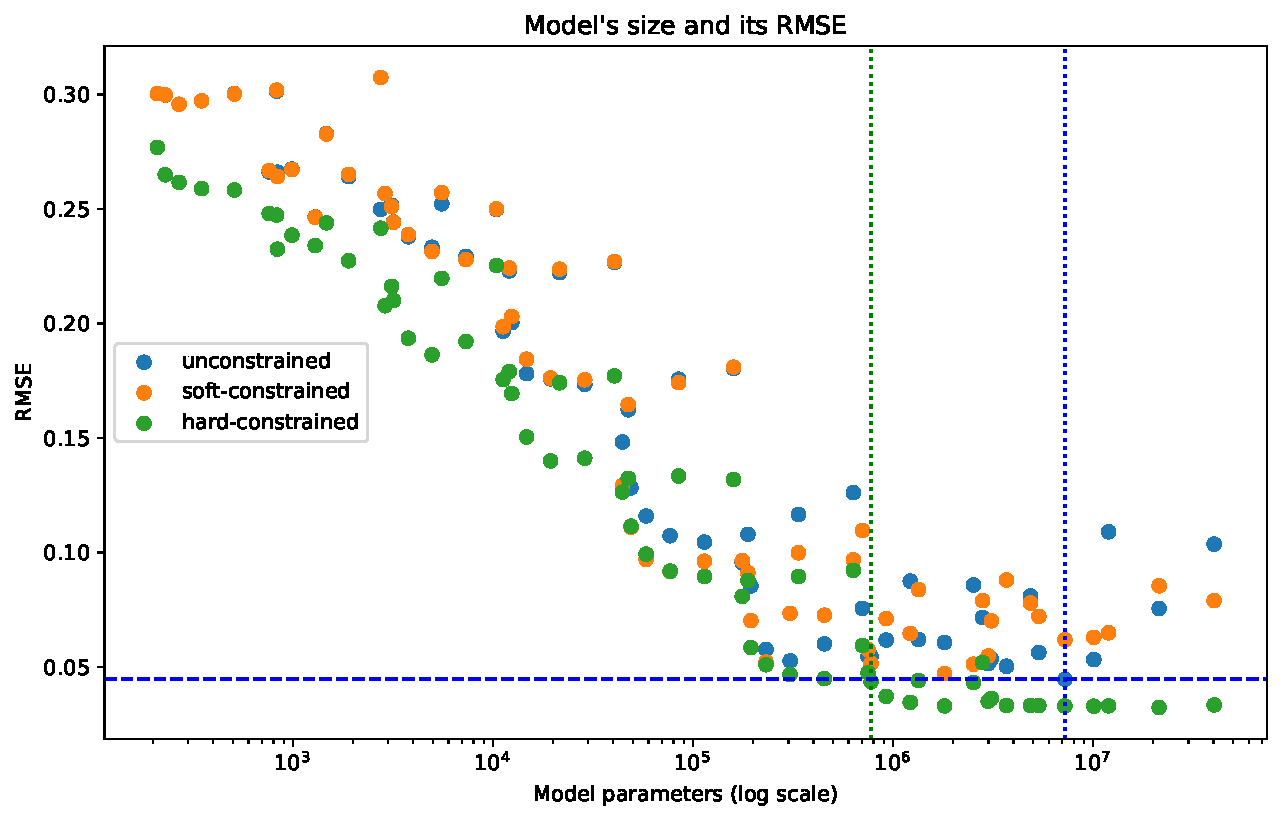
\includegraphics[width=\linewidth]{images/sizes_params.pdf}
    \caption[Model performance and the number of its parameters]{
    Model performance on the validation set and the number of its parameters.
    The lowest RMSE obtained by the unconstrained model is indicated by the blue dashed line, and its corresponding number of parameters is shown by the blue dotted line.
    The hard-constrained model that exceeds this performance while using the fewest learnable parameters is marked with the green dotted line.
    The graph thus suggests that applying a hard constraint can shrink the model size without degrading its performance.}
    \label{fig:sizes_params}
\end{figure}

\section{Evaluation on test data}
\label{s:test_eval}

In the previous experiments, the best improvement resulting from using the constraints was for the scale factor of $16$.
For this scale factor, the best performances on the validation set among the unconstrained, soft-constrained, and hard-constrained models are shown in Table~\ref{tab:val_bests}.

\begin{table}[h!]
    \centering
    \begin{tabular}{|m{0.25\linewidth}|m{0.2\linewidth}|m{0.2\linewidth}|m{0.2\linewidth}|}
        \hline
         \textbf{Model type} & \textbf{Resampling} & \textbf{Validation} \textbf{MAE} & \textbf{Validation} \textbf{RMSE} \\
         \hline \hline
         Unconstrained & cubic spline & 0.02983 & 0.04135 \\
         \hline
         Soft-constrained & average & 0.02709 & 0.0358 \\
         \hline
         Hard-constrained & average & 0.02603 & 0.0315 \\
         \hline
    \end{tabular}
    \caption[Best validation performances for different model types]{
    Best validation performances for different model types. 
    The best performance for the unconstrained model was achieved for the cubic spline resampling, whereas for the constrained models the average performed better. 
    All the best models had 128 features and 64 residual blocks.}
    \label{tab:val_bests}
\end{table}
\newpage
Now, the performance of the models that performed best on the validation set can be evaluated on unseen data from the ReKIS dataset, where we have target HR images.
For the unconstrained, soft-constrained, and hard-constrained models, the test MAE and RMSE metrics are shown in Table~\ref{tab:test_bests}.
We also calculated, for each pixel, the mean absolute error on the test set with the best hard-constrained model (Figure~\ref{fig:test_mae}).
In the referenced figure, the errors do not seem to be uniformly distributed and show a higher number of outliers, which is characteristic of training with absolute error.
A greater proportion of pixels showing higher mean absolute errors is found in the mountainous areas, where temperature downscaling is more challenging.
However, these pixels do not constitute a larger area and can be regarded as localized phenomena.

\begin{table}[h]
    \centering
    \begin{tabular}{|m{0.25\linewidth}|m{0.2\linewidth}|m{0.2\linewidth}|m{0.2\linewidth}|}
        \hline
         \textbf{Model type} & \textbf{Resampling} & \textbf{Test} \textbf{MAE} & \textbf{Test} \textbf{RMSE} \\
         \hline \hline
         Unconstrained & cubic spline & 0.02929 & 0.03886 \\
         \hline
         Soft-constrained & average & 0.02667 & 0.0338 \\
         \hline
         Hard-constrained & average & 0.02575 & 0.0306 \\
         \hline
    \end{tabular}
    \caption[Best test performances for different model types]{Best test performances for different model types. The best is the hard-constrained model. It is important to note that these models are the same as in Table~\ref{tab:val_bests}, only here the performance on test set is shown.}
    \label{tab:test_bests}
\end{table}

\begin{figure}[h]
    \centering
    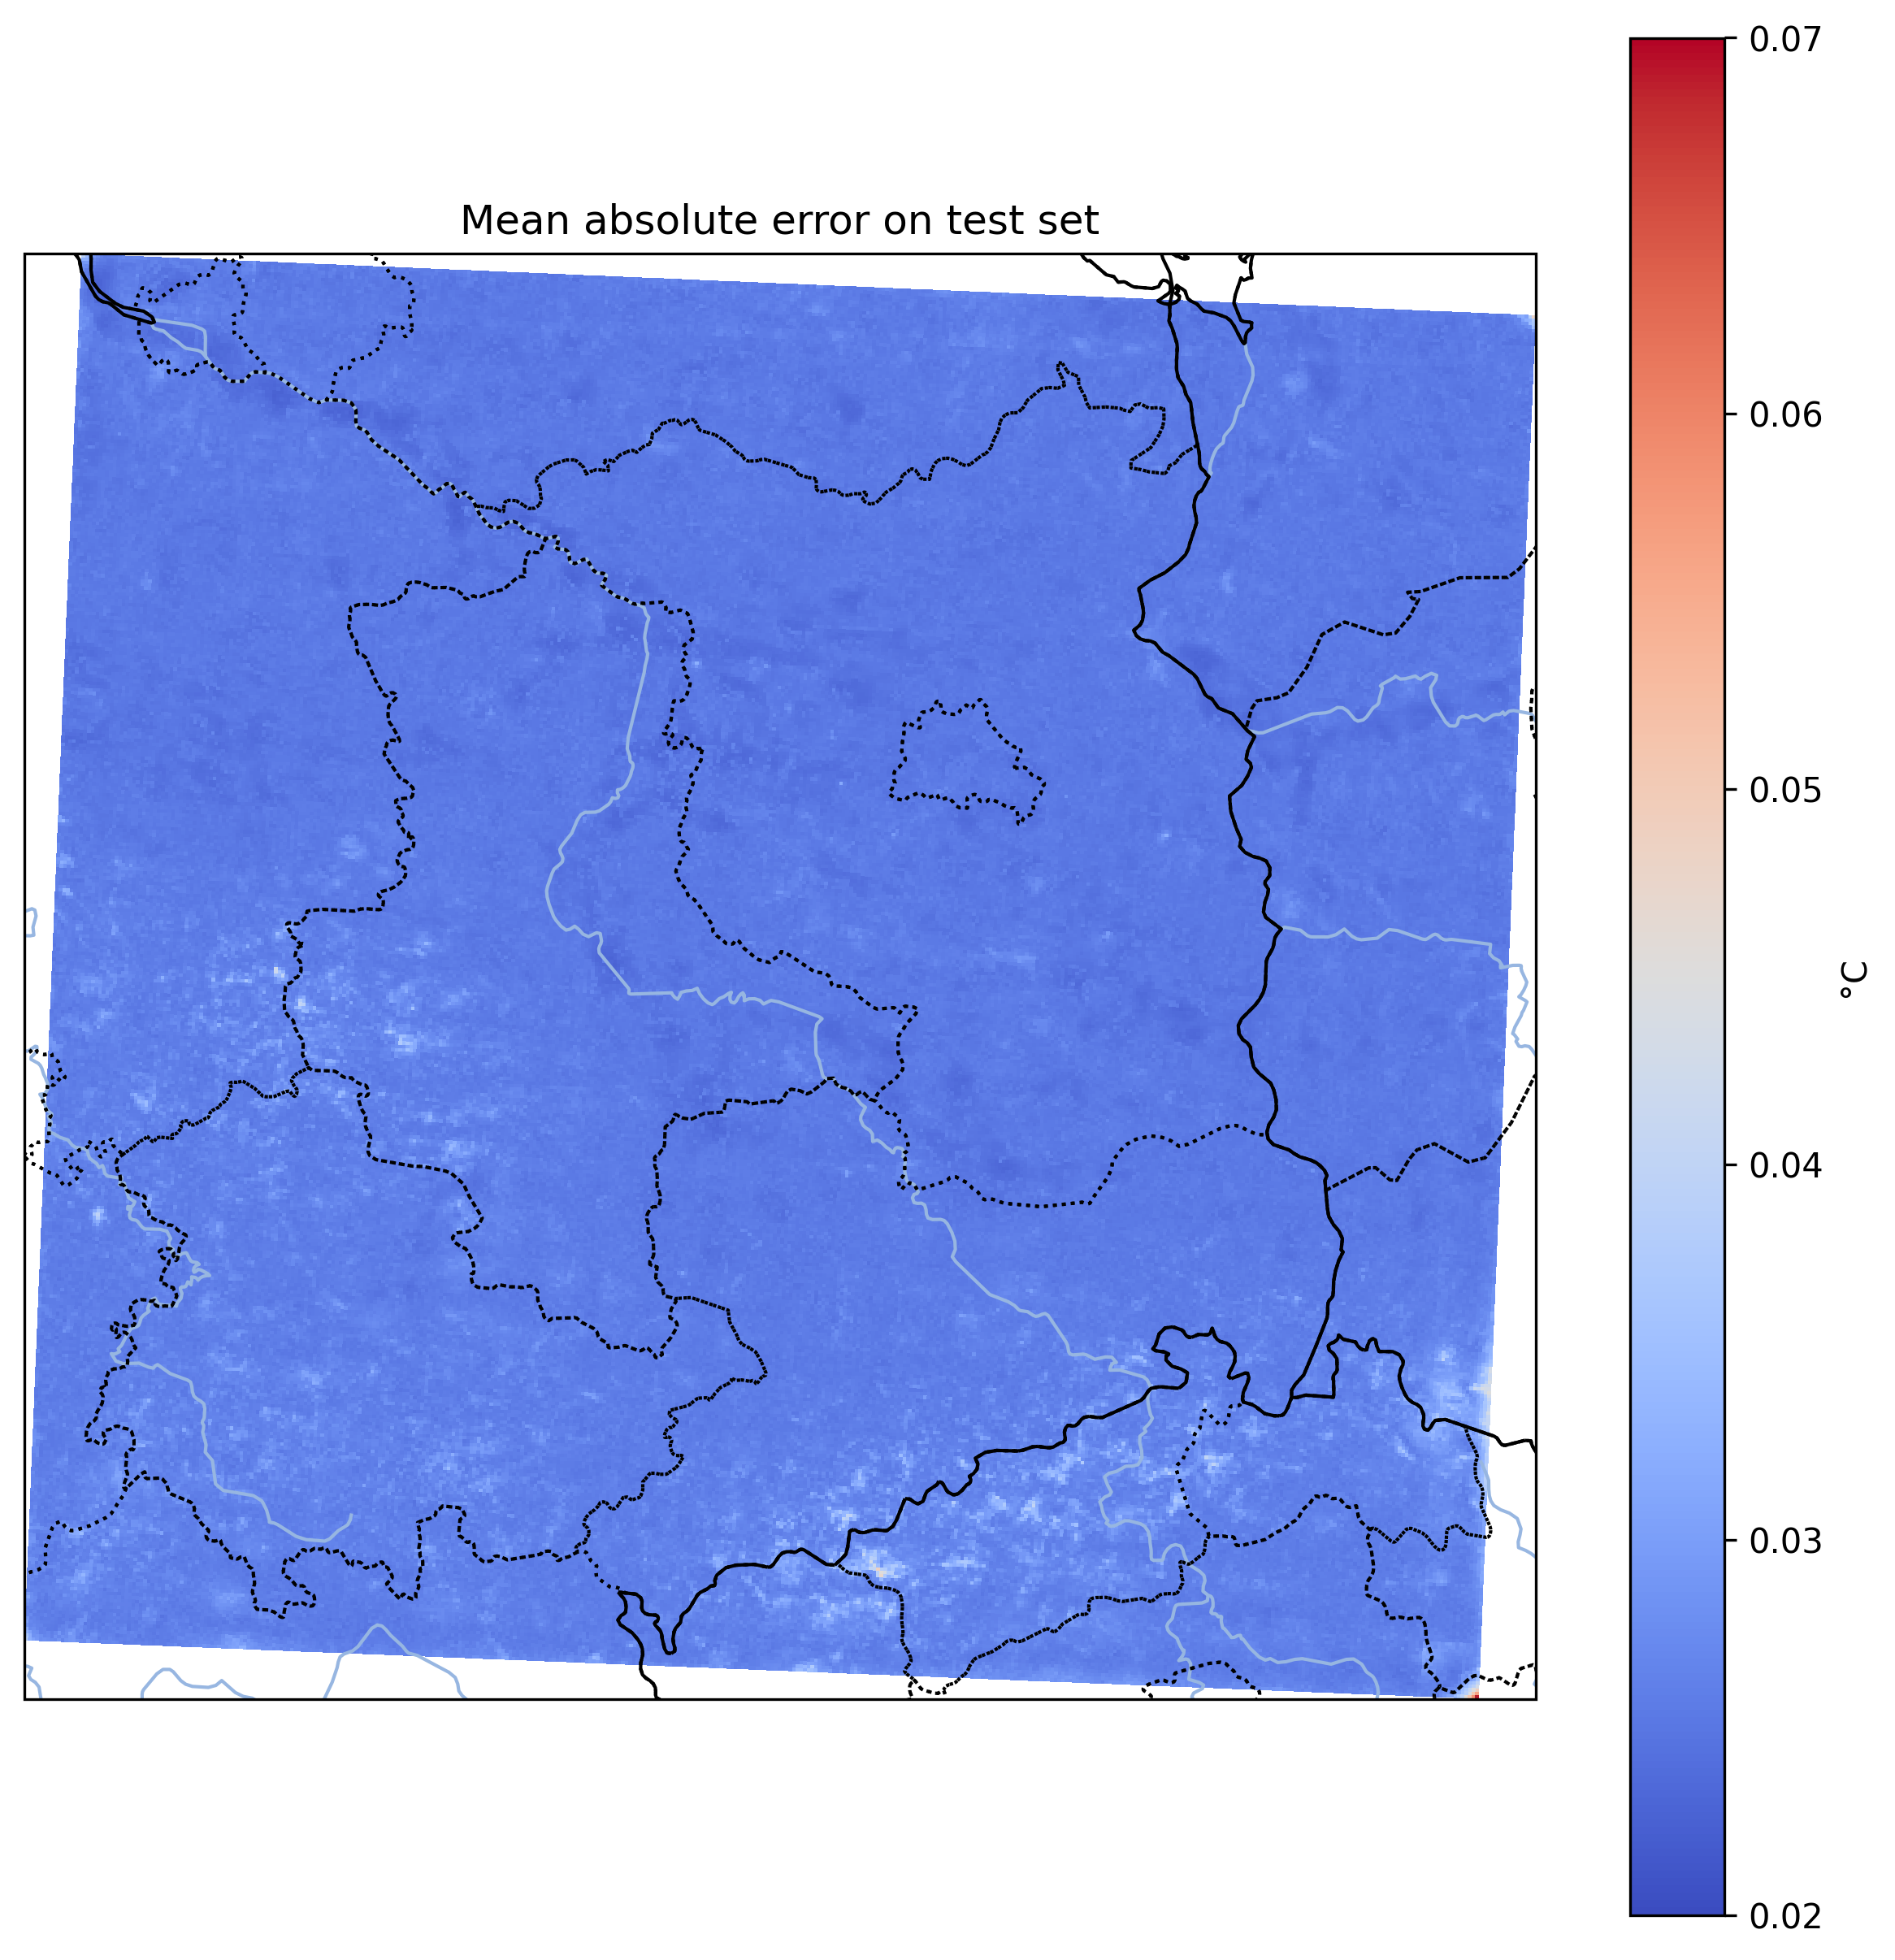
\includegraphics[width=0.5\linewidth]{images/mae.png}
    \caption[MAE on test set for the best model]{MAE on test set for the best model. The errors are not spread uniformly; only certain pixels exhibit large errors -- a characteristic pattern when training with an absolute-error loss function. The pixels that pose the greatest challenges for the model are found in the mountainous areas rather than in the plains.}
    \label{fig:test_mae}
\end{figure}

\section{Downscaling of EURO-CORDEX}

The best performance was measured (Section~\ref{s:test_eval}) in the setup of average resampling and the hard-constrained EDSR with 128 features and 64 residual blocks.
The EURO-CORDEX data must be reprojected to align with the CRS and resolution of the LR ReKIS data before being fed into the neural network.
After this procedure, they were downscaled using the above defined model.
The results are shown as visual examples in Figure~\ref{fig:downscaled_cordex}.
However, we are unable to further evaluate these results because no high-resolution EURO-CORDEX data are available.

\begin{figure}
    \centering
    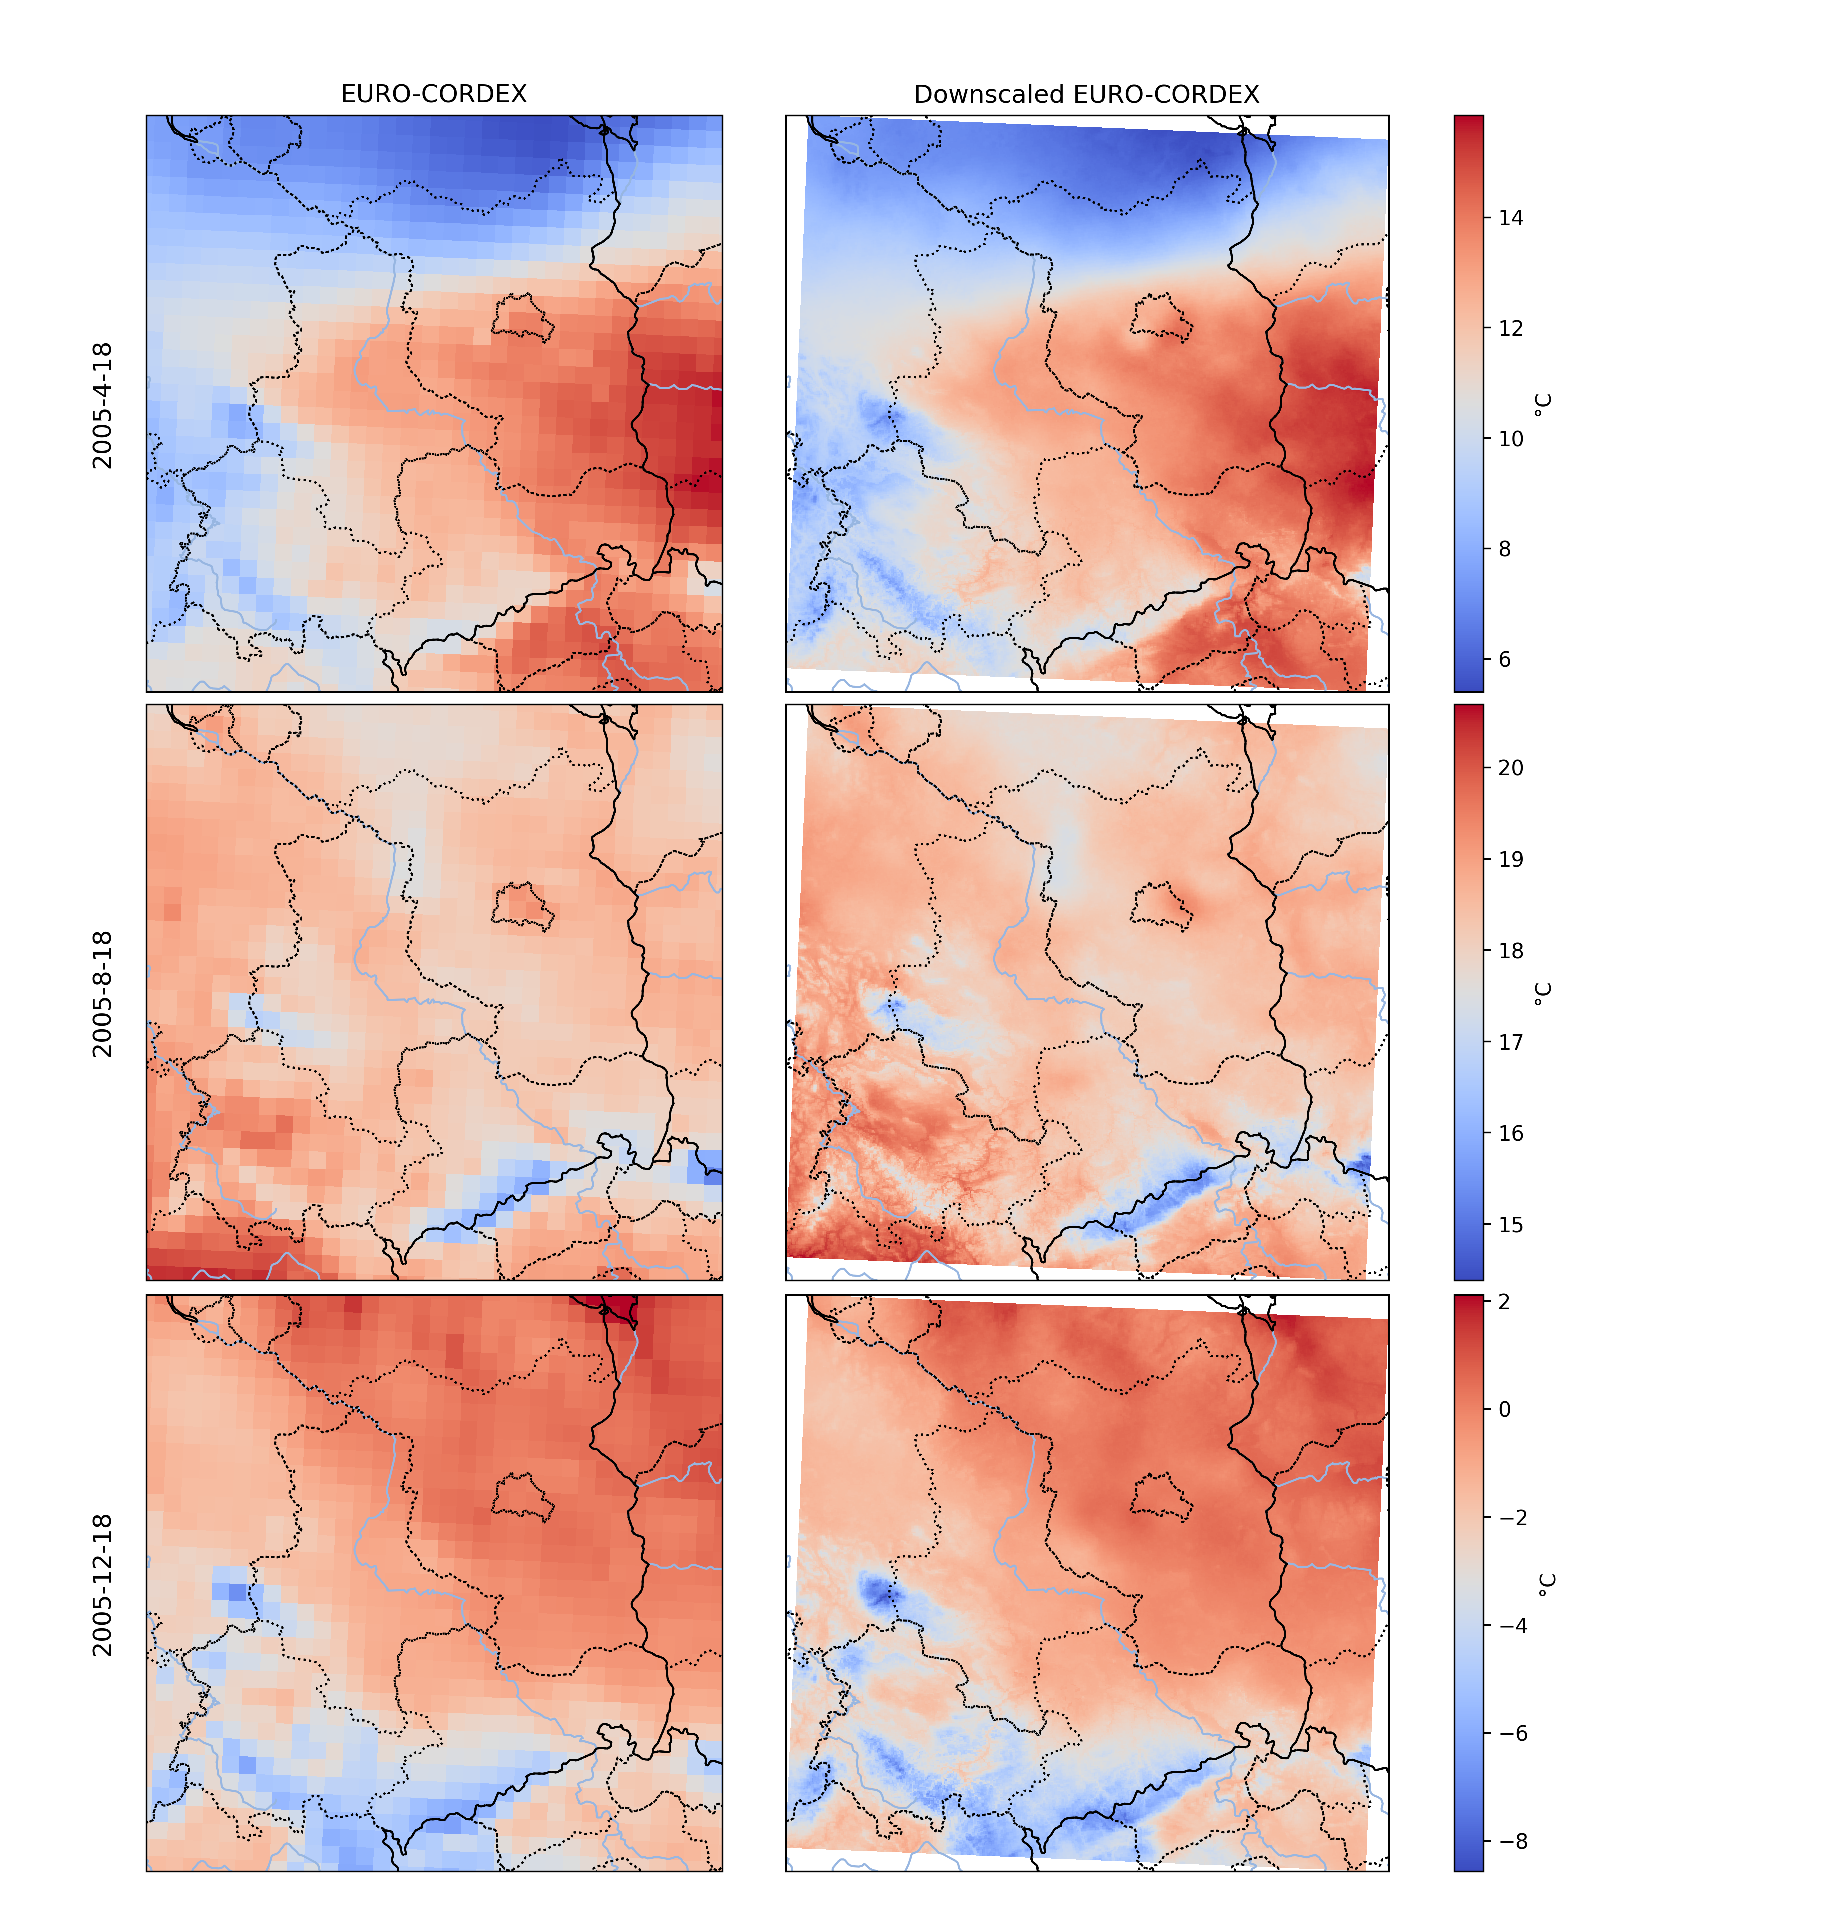
\includegraphics[width=\linewidth]{images/downscaled_cordex.pdf}
    \caption[Downscaling EURO-CORDEX]{
    Downscaling EURO-CORDEX. 
    On the left, images from the original resolution of EURO-CORDEX dataset are shown in the study region. 
    They are then upscaled so they can be used as input to our model, producing the images displayed on the right.
    The images are shown in distinct seasons.
    In April we can see a smooth transition from cold on the north to warmer weather in the central part of the region, which is smoother in the downscaled version.
    Across all displayed images, high-resolution features are mainly visible in the mountainous area in the southeastern part of the region and along the German-Czech border.
    Note that on the left, the EURO-CORDEX data cover all of Europe, while the downscaled dataset is limited to the ReKIS region, which results in the white areas along the sides.
    }
    \label{fig:downscaled_cordex}
\end{figure}
